%SETUP%
\documentclass[a4paper,11pt,oneside,titlepage]{book}
\usepackage[T1]{fontenc}		% Codifica dei font; T1 codifica di output dell'italiano e di lingue occidentali
\usepackage[utf8]{inputenc}		% Codifica degli input; abilita l'utilizzo di caratteri accentati
\usepackage[italian]{babel}		% Set the languages; the last one is the main language
\usepackage{geometry}			% Allow to change the margin
\usepackage{setspace}			% Allow to change the interline with \begin{onehalfspaceng} ecc.
\usepackage{fancyhdr}			% Fancy style for page layout
\usepackage{afterpage} 			% Allow to load blank pages with the command '\afterpage{\null\thispagestyle{empty}\clearpage}' 
\usepackage{hyperref}			% Crea collegamenti ipertestuali rendendo cliccabili i riferimenti
\usepackage{url}
\usepackage{color}			% Allow to use colors
\usepackage{xcolor}			% manage colors
\usepackage{enumerate}			% Numbered lists
\usepackage{enumitem}			% Allow to manage the style of the list
\usepackage{graphicx}			% Images
\usepackage{epstopdf}			% allows to convert eps images to pdf for use with pdflatex
\usepackage{pstool}			% Allows to use psfrag with pdflatex (no latex compiler needed)
\usepackage{psfrag}
%\usepackage[normal]{subfigure}		% manage subfigures
\usepackage{subfig}		% manage subfigures
\usepackage{array}			% Tables
\usepackage{tabularx}			% allow to set the width of the whole table
\usepackage[bottom]{footmisc}		% To attach footnote at the end of the page
\usepackage{booktabs}			% is a must for professional-looking layout
\usepackage{longtable}			% is very popular for multi-page tables
\usepackage{caption}			% Captions
\usepackage{float}			% Manage float objects (image, table, ecc.)
\usepackage{rotating}			% permette di ruotare immagini, tabelle, ecc. di 90° o di 270°
\usepackage{rotfloat}			% costruisce un ponte tra i pacchetti float e rotating
\usepackage{amsmath} 			% Equations
\usepackage{amssymb}			% Mathematical Symbols
\usepackage{cancel}                     % Simplification Cancellation
\usepackage{mleftright}
\usepackage{listings}   
\usepackage{caption}
\usepackage{subcaption}    
\usepackage{placeins}           
% Codes
\definecolor{lstgreen}{rgb}{0,0.6,0}
\definecolor{lstgray}{rgb}{0.5,0.5,0.5}
\definecolor{lstmauve}{rgb}{0.58,0,0.82}
\lstset{ %
  backgroundcolor=\color{white},   % choose the background color
  basicstyle=\footnotesize,        % size of fonts used for the code
  breaklines=true,                 % automatic line breaking only at whitespace
  captionpos=b,                    % sets the caption-position to bottom
  commentstyle=\color{lstgreen},    % comment style
  escapeinside={\%*}{*)},          % if you want to add LaTeX within your code
  keywordstyle=\color{blue},       % keyword style
  stringstyle=\color{lstmauve},     % string literal style
}
%\usepackage{vector}  			% Allows "\bvec{}" and "\buvec{}" for "blackboard" style bold vectors in maths
\usepackage[swapnames,norules,nouppercase]{frontespizio}
\usepackage[intoc]{nomencl}
\usepackage[acronym,toc,nomain,nopostdot,nonumberlist]{glossaries}
\usepackage[square, numbers, comma, sort&compress]{natbib}
\usepackage{verbatim}                   % Needed for the "comment" environment to make LaTeX comments
\usepackage{wrapfig}                 % Per inserire le figure contornate da testo
\usepackage{blindtext}
\geometry{a4paper,top=2.5cm,bottom=2.5cm,left=2cm,right=2cm,heightrounded,bindingoffset=5mm,headheight=13.6pt}
% -------------------------------------- Line-spacing --------------------------------------- %
\linespread{1.2} 
%\linespread{1.5} 
%\linespread{2} 
%\raggedbottom % disattiva lo 'stiracchiamento' del testo; va a favore di spazio bianco a fondo pagina
% ---------------------------------------- Numeration --------------------------------------- %
%\setcounter{secnumdepth}{3} % set the enumeration of the sections
%\setcounter{tocdepth}{3}    % set the enumeration of the sections in the table of contents
%--------------------------------------- Page layout -----------------------------------------%
%\pagestyle{fancy}                       % definisce lo stile di pagina aprendo la strada al pacchetto fancyhdr
%\renewcommand{\chaptermark}[1]{\markright{\chaptername\ \thechapter.\ #1}{}}    % ridefinisce la macro \rightmark per i capitoli
%\renewcommand{\sectionmark}[1]{\markright{\sectionname\ \thesection.\ #1}}      % ridefinisce la macro \rightmark per le sezioni
%\renewcommand{\sectionmark}[1]{\markright{\thesection.\ #1}}
%\lhead{Giacomo Della Posta}             % in alto a sinistra
%\chead{}                                % in alto al centro
%\rhead{\slshape \rightmark}             % in alto a destra (\rightmark contiene ...)
%\lfoot{Giacomo Della Posta}             % in basso a sinistra
%\cfoot{\thepage}                        % in basso al centro (\thepage per mettere il numero di pagina)
%\rfoot{}                                % in basso a destra
%\renewcommand{\headrulewidth}{0.4pt}    % spessore della linea di separazione in alto (0 per eliminare la linea)
%\renewcommand{\footrulewidth}{0.4pt}    % spessore della linea di separazione in basso (0 per eliminare la linea)
\fancypagestyle{plain}{%                                        % modifica dello stile predefinito plain
                        \fancyhf{}                       % cancella tutti i campi di  intestazione e pie di pagina
                        \fancyfoot[R]{\thepage}                 % mette al centro il numero di pagina
                        \renewcommand{\headrulewidth}{0pt}      % spessore della linea di separazione in alto (0 per eliminare la linea)
                        \renewcommand{\footrulewidth}{0.4pt}    % spessore della linea di separazione in basso (0 per eliminare la linea)
                        }                                       % modifica dello stile predefinito plain
\captionsetup{font=small,labelfont=bf,textfont=normalfont,tableposition=bottom,figureposition=bottom}
%\captionsetup{font=small,labelfont=bf,textfont=bf,tableposition=bottom,figureposition=bottom}
% ---------------------------------------- Itemize ------------------------------------------ %
%\setlist[itemize]{noitemsep, topsep=0pt} %Se non vuoi i pallini degli elenchi vuoti, allora commenta queste linee      
%\renewcommand{\labelitemi}{$\circ$}	% items i with empty bullets
%\renewcommand{\labelitemii}{$\bullet$}	% items ii with black bullets
\hypersetup{colorlinks=true, linkcolor=black, citecolor=black, filecolor=black, urlcolor=black}
\definecolor{red-univaq}{RGB}{130,36,51} % example \definecolor{name}{model}{color-spec}
\definecolor{univaq}{RGB}{242,195,80} % example \definecolor{name}{model}{color-spec}
\makenomenclature % Generate the nomenclature
\makeglossaries % Generate the glossary
%\lstset{language=[90]Fortran,
%        inputpath=/home/luca/PhD/Thesis/Code,
%        basicstyle=\small\ttfamily, 
%        xleftmargin=0cm,
%        fontadjust=true,
%        keepspaces=true,
%        basewidth=0.5em,
%        breakatwhitespace=false,           % sets if automatic breaks should only happen at whitespace
%        breaklines=false,                  % sets automatic line breaking
%        captionpos=b,                     % b=bottom
%        backgroundcolor=\color{white},
%        identifierstyle=\color{black},
%\bibliographystyle{abbrv} % abbrv --> [1], [2], ecc.
\bibliographystyle{unsrtnat} 
% ---------------------------------------- Dedication ------------------------------------------ %
\newenvironment{dedication}
{
  \phantom{.}
  \vspace{13cm}
  \begin{quote} \begin{flushright}}
{\end{flushright} \end{quote}}
\usepackage{calligra}

\begin{document}

%   FRONT MATTER                                            %
\frontmatter 	   % Begin Roman style (i, ii, iii, iv...) page numbering
\pagestyle{empty}  % No headers or footers for the following pages

%   TITLE PAGE
\begin{frontespizio}
% Remember: After editing this file, delete the cache and recompile
%---------------------Definizione font---------------------%
\Preambolo{\renewcommand{\fronttitlefont}{\fontsize{24}{24}\bfseries}}
%----------------------------------------------------------%
	% \frontinstitutionfont 	Neretto, 14/17 
	% \frontdivisionfont 		Tondo, 12/16 
	% \frontpretitlefont 		Maiuscoletto, 10/12
	% \fronttitlefont 		Neretto, 17/21 
	% \frontsubtitlefont 		Tondo, 12/14
	% \frontfixednamesfont 		Tondo, 12/14 
	% \frontnamesfont 		Neretto, 12/14 
	% \frontsmallfont 		Neretto, 9/11 
	% \frontfootfont	 	Neretto, 12/14 

	% \bfseries	Grassetto
	% \itshape	Corsivo
	% \scshape	Maiuscoletto
%----------------------------------------------------------%
\Margini{4cm}{3cm}{3cm}{3cm} % Margini sinistro, in basso, destro e in alto
\Logo[4cm]{figures/logo/UnivAQ_logoA.eps}
%\Universita{L'Aquila}
\Istituzione{Dipartimento di Ingegneria e Scienze dell'Informazione e Matematica}
%\Divisione{Department of Information Engineering, Computer Science and Mathematics}	% ENG
\Divisione{Tesi di Laurea Triennale in Informatica}		% ITA
%\Dipartimento{Dipartimento di Ingegneria e Scienze dell'Informazione e Matematica}
%\Corso[Master Degree]{Ingegneria delle Telecomunicazioni}
\Scuola{}
\Titoletto{}

\Titolo{Progettazione e sviluppo di un assistente virtuale di cucina in realtà mista}
%\Sottotitolo{}

\Punteggiatura{} % Modifica la punteggiatura dopo 'Candidato', 'Realatore' ecc. (vuoto per togliere)
\NCandidato{Laureando} % Sostituisce 'Candidato' con '...'
\Preambolo{\renewcommand{\frontsmallfont}[1]{\small}}
\Candidato[278662]{Giacomo Paolocci}

%\NRelatore{Thesis Advisor}{Relatori}
\NRelatore{Relatore}{Relatori}
\Relatore{Prof. Francesco Tarquini}
%\NCorrelatore{Thesis Co-Advisor}{Relatori}
\NCorrelatore{Correlatore}{Relatori}
\Correlatore{Dr. Leonardo D'Errico}
%\Rientro{1cm} % Rientro di Relatore e Candidato

\Piede{Anno Accademico 2024-2025}
\end{frontespizio}

\IfFileExists{\jobname-frn.pdf}{}{%
\immediate\write18{pdflatex \jobname-frn}} 
\clearpage

%   TOC - LOF - LOT
\begin{singlespace}
 \tableofcontents 	
% \renewcommand{\lstlistlistingname}{List of Code}
% \addcontentsline{toc}{chapter}{\lstlistlistingname} 
% \lstlistoflistings

%   NOMENCLATURE AND ACRONYMS
 \printnomenclature
 \printglossaries
\end{singlespace}

%   MAIN MATTER
\mainmatter	  % Begin normal, numeric (1,2,3...) page numbering
\clearpage
% ------ set page style fancy with the follow 
\pagestyle{fancy} 
\renewcommand{\chaptermark}[1]{\markright{\chaptername\ \thechapter.\ #1}{}}
\renewcommand{\sectionmark}[1]{\markright{\thesection.\ #1}}
\lhead{} 
\chead{}                   
\rhead{\slshape \rightmark} 
\lfoot{Name}
\cfoot{} 
\rfoot{\thepage}          
\renewcommand{\headrulewidth}{0.4pt} 
\renewcommand{\footrulewidth}{0.4pt} 

%   CHAPTERS
\chapter{Introduzione}
\pagestyle{plain}
Questa tesi si propone di esplorare l'uso della Realtà Mista (MR) in un contesto culinario, con particolare attenzione all'uso di visori come gli HoloLens 2.\\ L'obiettivo principale è quello di sviluppare un'applicazione che possa aiutare a creare ricette con ingredienti inutilizzati evitando anche lo spreco alimentare. Tutto ciò riassunto in un'applicazione semplice e intuitiva che utilizza la MR per sovrapporre informazioni digitali al mondo reale, così da avere pieno controllo di quello che si fa e allo stesso tempo avere le mani libere da qualsiasi dispositivo fisico.\\
L'applicazione è stata sviluppata utilizzando Unity e il Mixed Reality Toolkit (MRTK), che forniscono gli strumenti necessari per creare esperienze MR. Inoltre, utilizzando L'LLM Google Gemini è possibile generare ricette in base agli ingredienti disponibili facendo una semplice foto, rendendo l'applicazione ancora più utile e versatile.
\begin{figure}[]
    
\includegraphics{figures/chapter_1/Windows_Mixed_Reality_logo.png}
    \centering
\end{figure}



\chapter{Tecnologie Utilizzate}
\pagestyle{plain}


\section{Realtà Mista (MR)}

\subsection{Storia}
Lo studio di tecnologie simili a realtà aumentata (AR), realtà mista (MR) e realtà virtuale (VR) risalgono alla fine degli anni '50, in particolare nel 1957 Morton Heiling sviluppò un simulatore, grande quanto un cabinato per videogiochi, che permetteva all'utilizzatore di visualizzare immagini 3d stereoscopiche, integrando l'esperienza con vento artificiale, vibrazioni, audio stereo e addirittura un dispositivo per la creazione di profumi.\\Ma l'applicazione che si avvicina di più a qualcosa di moderno arriva dall'utilizzo in aviazione, in particolare un sistema chiamato "Sword of Democles", un primo casco dotato di lenti per l'AR. Questo dispositivo serviva ad aiutare i piloti di elicottero ad atterrare di notte azionando le telecamere con l'utilizzo della testa. Un problema di questo dispositivo era il peso eccessivo, e da questo deriva proprio il suo nome. \\ Lo sviluppo continua nel 1992 con Loui B. Rosenberg con lo sviluppo del primo sistema AR immersivo che permetteva di guidare bracci robotici, tecnologia successivamente utilizzata nell'aeronautica militare statunitense. \cite{OverviewofAugmentedReality}
\\ In tempi recenti abbiamo visto lo sviluppo dei Google Glass, usciti nel 2013 e ritirati dal mercato nel 2023 \cite{EndofGoogleGlass}, e dei primi visori di realtà virtuale come l'Oculus Rift CV1, uscito nel 2016 \cite{OculusRift1}, che hanno creato le basi per visori più recenti come il Meta Quest 3 e gli Hololens 2, quest'utimi utilizzati proprio per la realizzazione di questa tesi.

\subsection{Definizione}
La realtà mista sovrappone al mondo fisico elementi tridimensionali con cui l'utente può interagire. Si contraddistingue per l'uso di un dispositivo, solitamente un visore, che tramite appositi sensori, riconosce e mappa tridimensionalmente l'ambiente circostante. Questo permette di inserirvi oggetti tridimensionali, con i quali l'utente interagisce grazie alla comprensione dei movimenti di mani, occhi e degli input vocali.
\begin{figure}[H]
    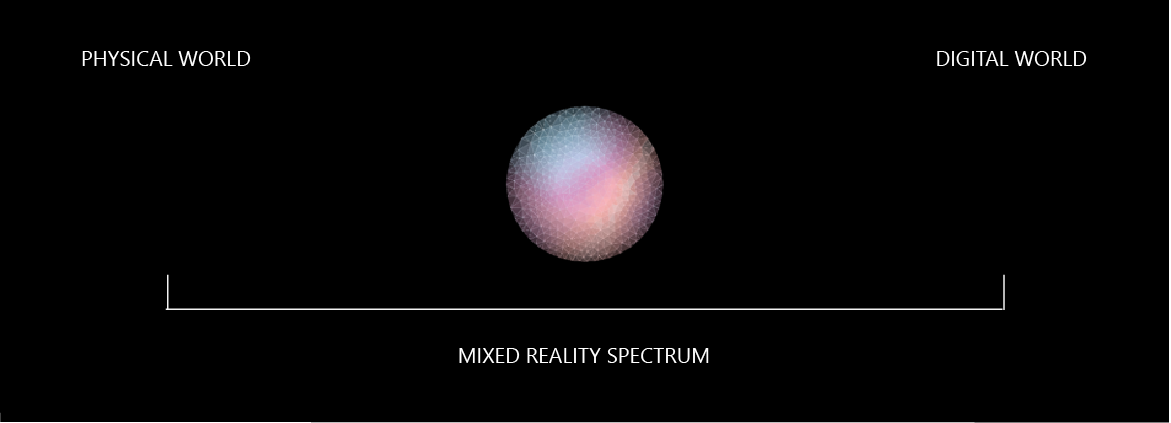
\includegraphics[scale=0.4]{figures/chapter_1/mixedrealityspectrum-worlds.png}
    \caption{Rappresentazione della fusione del mondo fisico con il mondo digitale nella realtà mista.}
    \centering
\end{figure}

Per consentire una esperienza immersiva fra realtà e oggetti 3d, chiamati anche ologrammi in ambito Microsoft, è emersa una nuova disciplina chiamata "HIC" o anche "Human-Computer Interaction", che si occupa di studiare come interagire virtualmente con il computer, ad esempio tramite tastiere, mouse, comandi vocali o tracciamenento dei movimenti. \cite{MixedRealityDefinition}

\begin{figure}[H]
    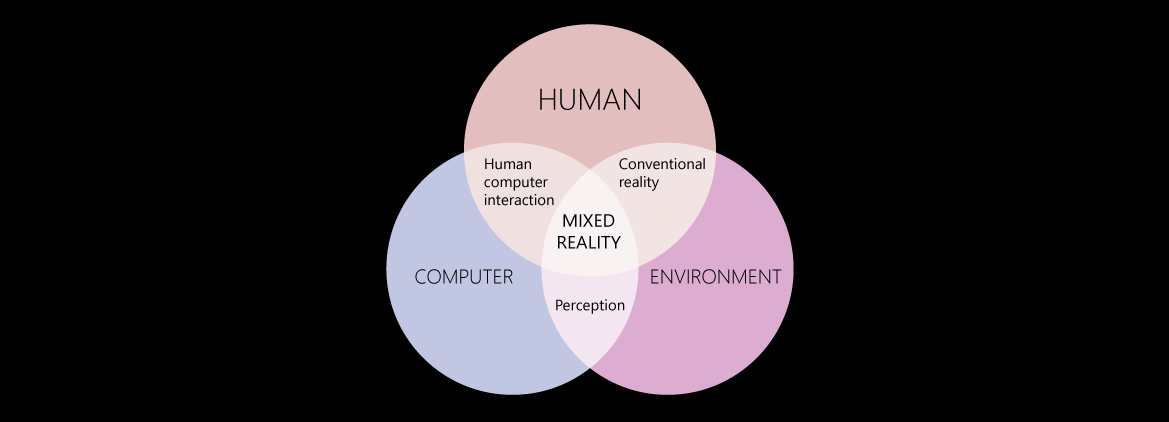
\includegraphics[scale=0.4]{figures/chapter_1/mixed-reality-venn-diagram.png}
    \caption{interazioni tra computer, utente e ambiente circostante.}
    \centering
\end{figure}
    
\subsection{Casi d'uso}
\subsubsection{Formazione di piloti in aereounatica}
Tramite l'utilizzo della realtà mista è possibile fare delle lezioni interattive simulate, ad esempio la risoluzione di un guasto all'impianto elettrico visualizzando in realtà mista la schematica dell'impianto, oppure illustrare ed allenare ad un'ispezione esterna dell'aereo. In questo ultimo caso lo studente, in una stanza abbastanza grande, può camminare intorno al modello 3d in scala dell'aereo, venendo aiutato dalla applicazione in MR durante le varie azioni di controllo, ad esempio la rotazione di maniglie o apertura di porte.\cite{MixedRealityUseCasesforPilotTraining}

\subsubsection{Formazione e simulazione in ambito industriale}
La realtà aumentata offre un modo efficace e sicuro per imparare attraverso la pratica, soprattutto in situazioni potenzialmente pericolose. Grazie a simulazioni immersive, i tirocinanti possono affrontare scenari realistici senza correre rischi reali, ricevendo feedback immediato sui propri errori. Questo tipo di formazione unisce la percezione dell'ambiante reale con l'attività virtuale, permettendo di sviluppare competenze pratiche senza creare danni a persone o macchinari \cite{MicrosoftTrainingandSimulationforEnterprises}
\begin{figure}[H]
    \centering
    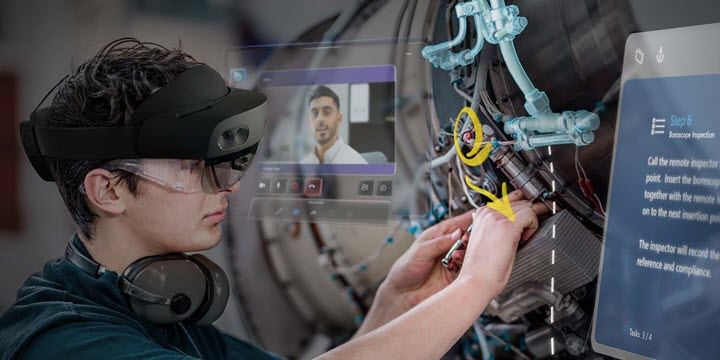
\includegraphics[width=0.5\textwidth,height=0.5\textheight,keepaspectratio]{figures/chapter_1/hololens_in_azienda.jpg}
    \caption{Utilizzo della realtà aumentata in ambito industriale}
\end{figure}

\subsubsection{Prototipazione e produzione per le imprese}
L'integrazione della realtà aumentata nei processi di prototipazione e produzione può portare a una significativa riduzione dei costi, soprattutto su scala industriale. Spostare la progettazione in uno spazio virtuale consente di evitare la produzione di prototipi fisici costosi e di velocizzare l'intero ciclo di sviluppo grazie a iterazioni rapide e meno dispendiose. Questo approccio non solo ottimizza le tempistiche, ma migliora anche la precisione nella produzione, aumentando la sicurezza e l'affidabilità delle linee produttive. In molti casi, l'introduzione della realtà aumentata ha portato benefici concreti in termini di stabilità delle infrastrutture, sicurezza dei lavoratori e qualità del prodotto finale.\cite{MicrosoftPrototypingforEnterprises}

\subsubsection{Musei e mostre virtuali}
La realtà virtuale si è dimostrata uno strumento potente per il mondo dei musei, delle mostre d'arte e d'intrattenimento, dei servizi di hosting di eventi, dei servizi turistici e di altre attività e servizi simili incentrati sulle mostre \cite{MicrosoftVirtualMuseums}. In particolare l'utilizzo della realtà mista in ambienti reali consente una perfetta armonia tra il mondo reale e quello virtuale, permettendo di visualizzare opere d'arte o reperti storici in 3d, con la possibilità di interagire con essi. \cite{MixedRealityinMuseums}

\section{Hardware}
Fra i vari visori di realtà mista, il più utilizzato è l'HoloLens 2, un visore sviluppato da Microsoft, che permette di visualizzare ologrammi in 3d e interagire con essi tramite comandi vocali, movimenti delle mani e tracciamento degli occhi. 
\subsection{HoloLens 2}
Gli HoloLens 2, successori degli HoloLens 1, sono visori di realtà mista sviluppati da Microsoft e rilasciati nel 2019, sono dotati di un display olografico che consente di sovrapporre oggetti virtuali al mondo reale e si basano sul sistema operativo "Windows Holographic OS" derivato da Windows 10

\begin{figure}[H]
    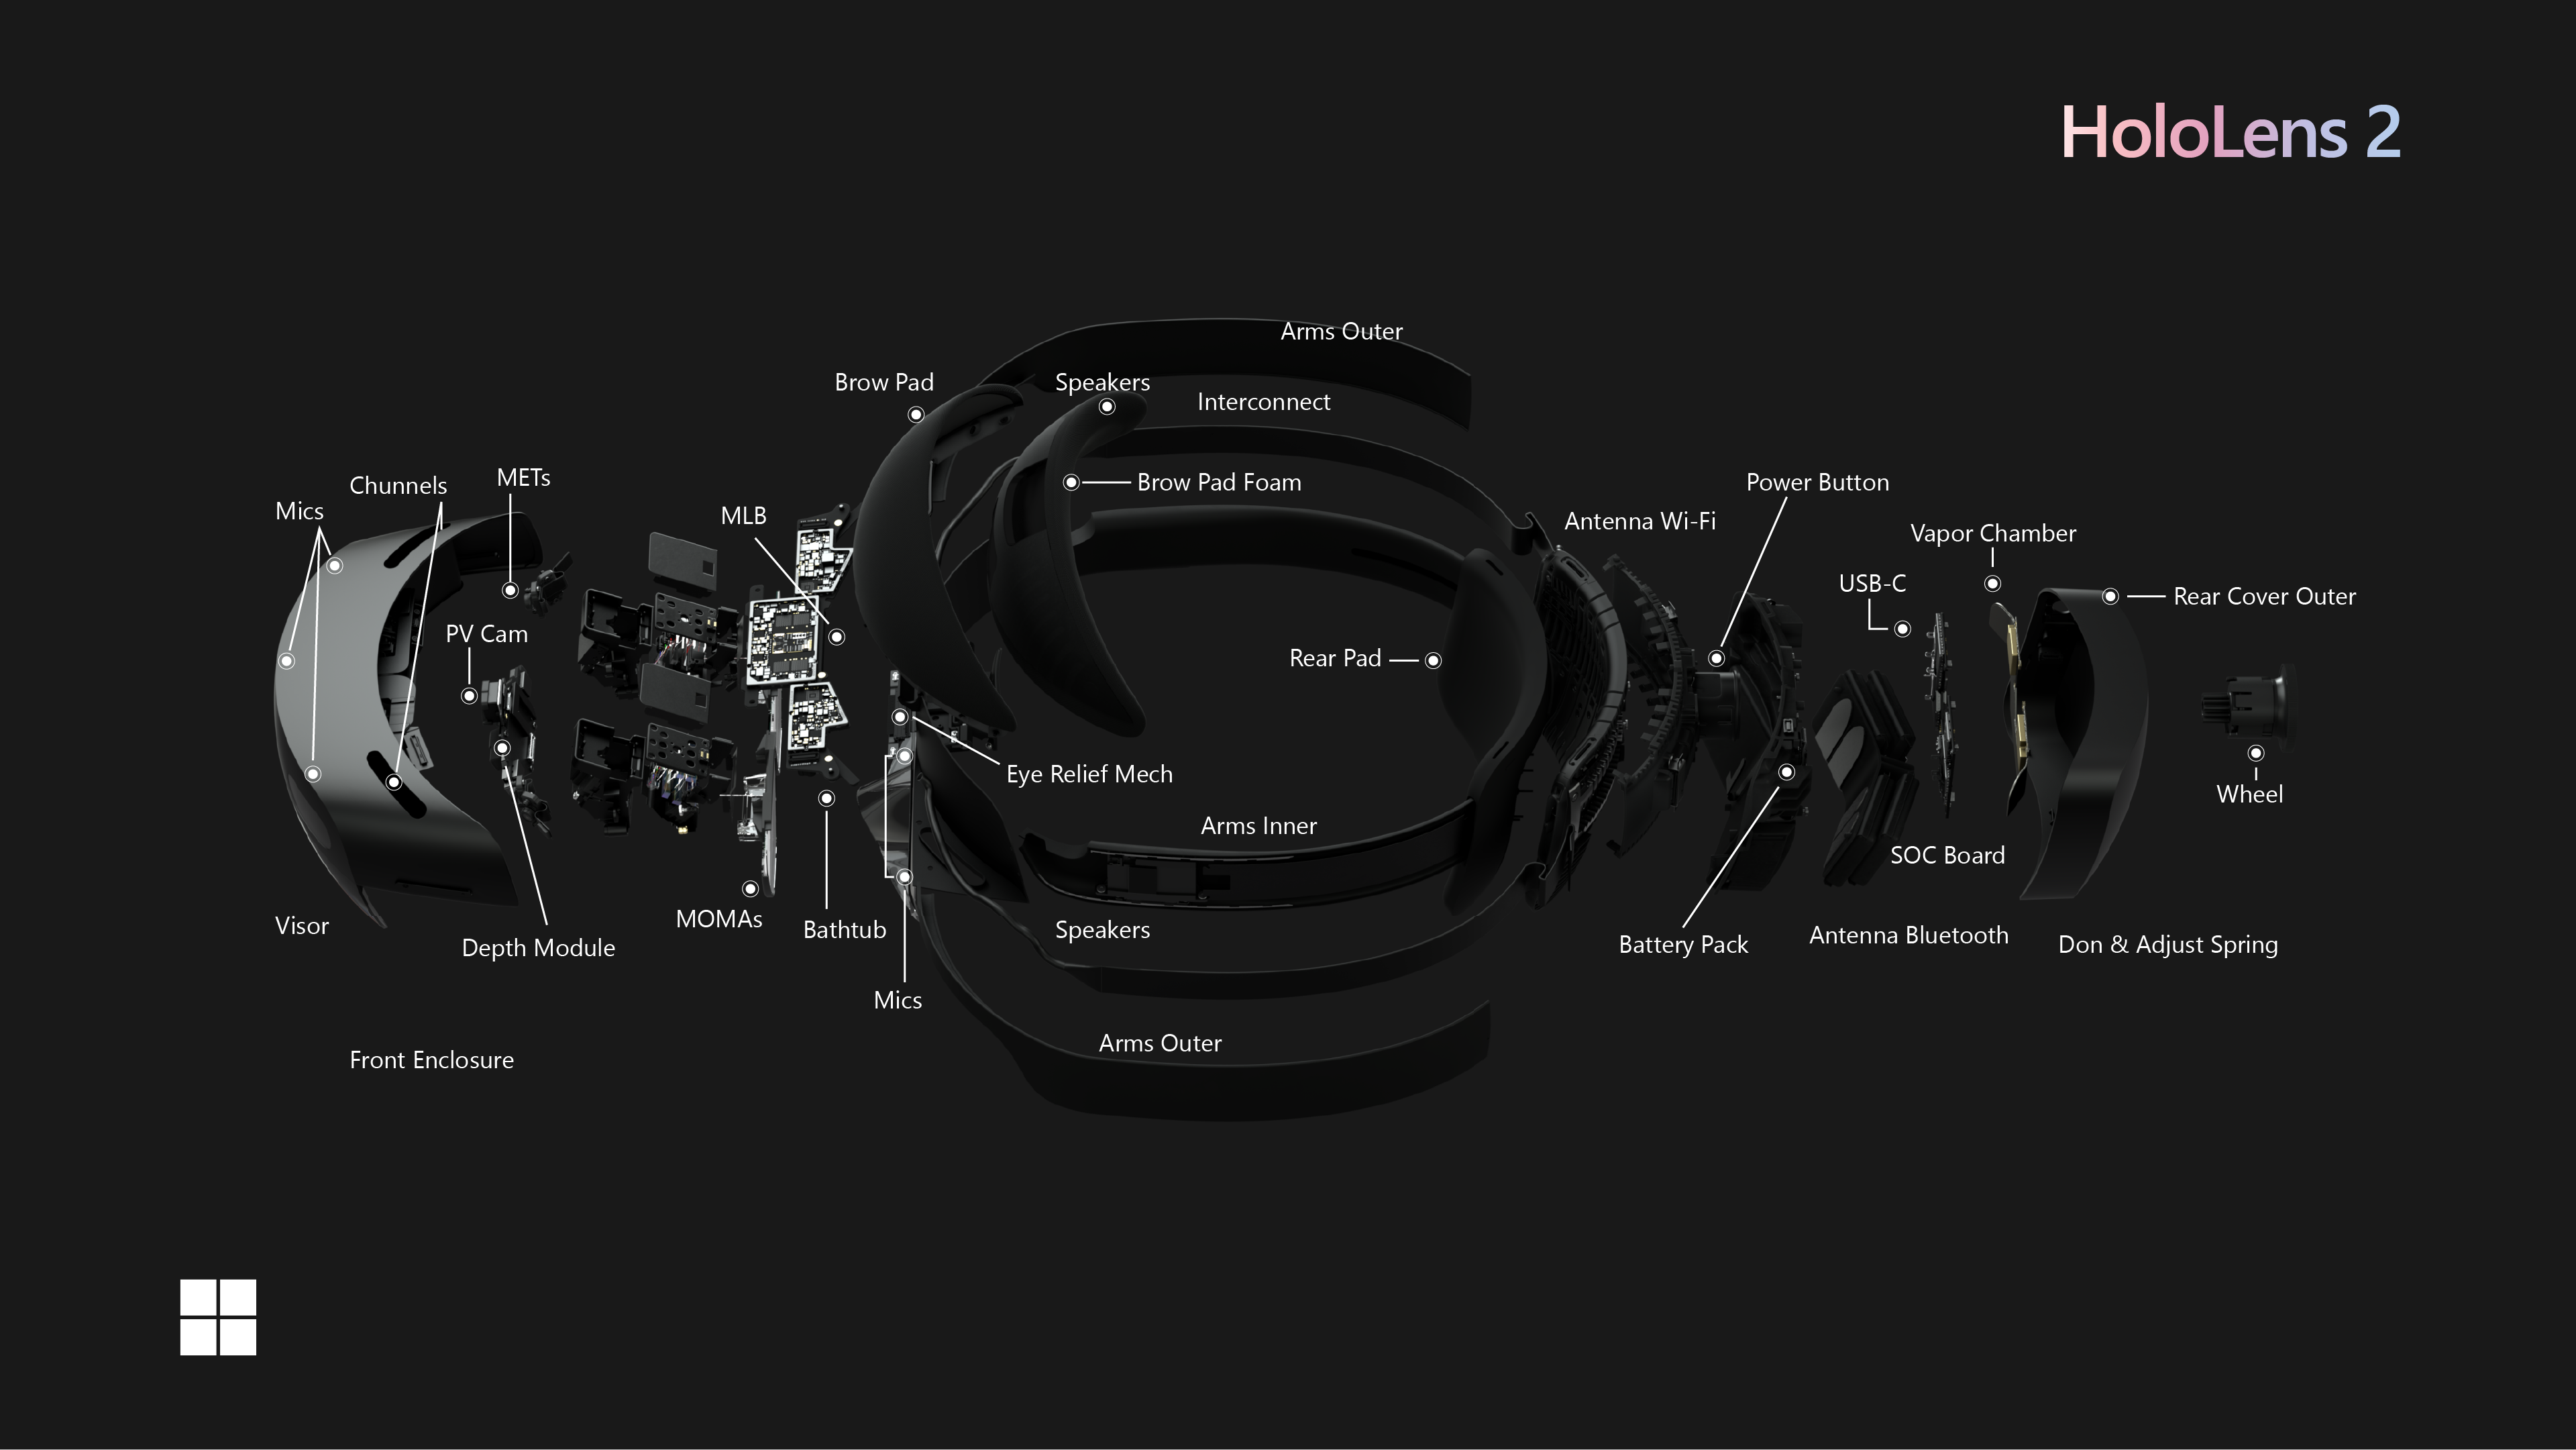
\includegraphics[width=\textwidth,height=\textheight,keepaspectratio]{figures/chapter_1/hololens2-exploded-view-diagram.png}
    \caption{Esplosione 3d del visore HoloLens 2}
    \centering
\end{figure}
Come si può vedere in figura tutta la parte di elaborazione di trova nella parte posteriore del visore, mentre nalla parte anteriore troviamo l'hardware per la proiezione degli ologrammi, i sensori come giroscopio e accelerometro, e le telecamera che permettono il tracciamento delle mani e degli occhi.In particolare abbiamo 4 telecamere frontali per il riconoscimento dell'ambiente circostante, 2 telecaere a infrarossi per il tracciamento oculare e una fotocamera frontale a colori da 8megapixel.\\
Il visore è dotato di un processore Qualcomm Snapdragon 850, 4 GB di RAM e 64 GB di memoria interna, la batteria ha una durata di circa 2-3 ore. Il visore è dotato di un sistema audio spaziale e di un microfono a 5 canali usati anche per il riconoscimento vocale. \cite{WhatIsHoloLens}\\
Per questo progetto è stato adottato questo visore solo perchè offriva l'accesso alla telecamera frontale,cosa non disponibile in altri visori come il Meta Quest 3, oltre al fatto di essere quello di più recente produzione da parte di Microsoft. 

\section{Software e AI}
Per la realizzazio del progetto sono stati utilizzati il motore grafico Unity, il Mixed Reality Toolkit (MRTK) e Google Gemini.

\subsection{Unity}
Unity è un motore grafico multipiattaforma sviluppato da Unity Technologies, utilizzato per la creazione di videogiochi e applicazioni in 2D e 3D. È particolarmente popolare per lo sviluppo di giochi per dispositivi mobili, console e PC. Nel nostro caso è stato utilizzato per la creazione di un'applicazione di realtà mista per gli HoloLens 2 utilizzando il Mixed Reality Toolkit (MRTK) e il linguaggio di programmazione C\#.
\subsubsection{Overview di Unity} 
\begin{figure}[H]
    \centering
    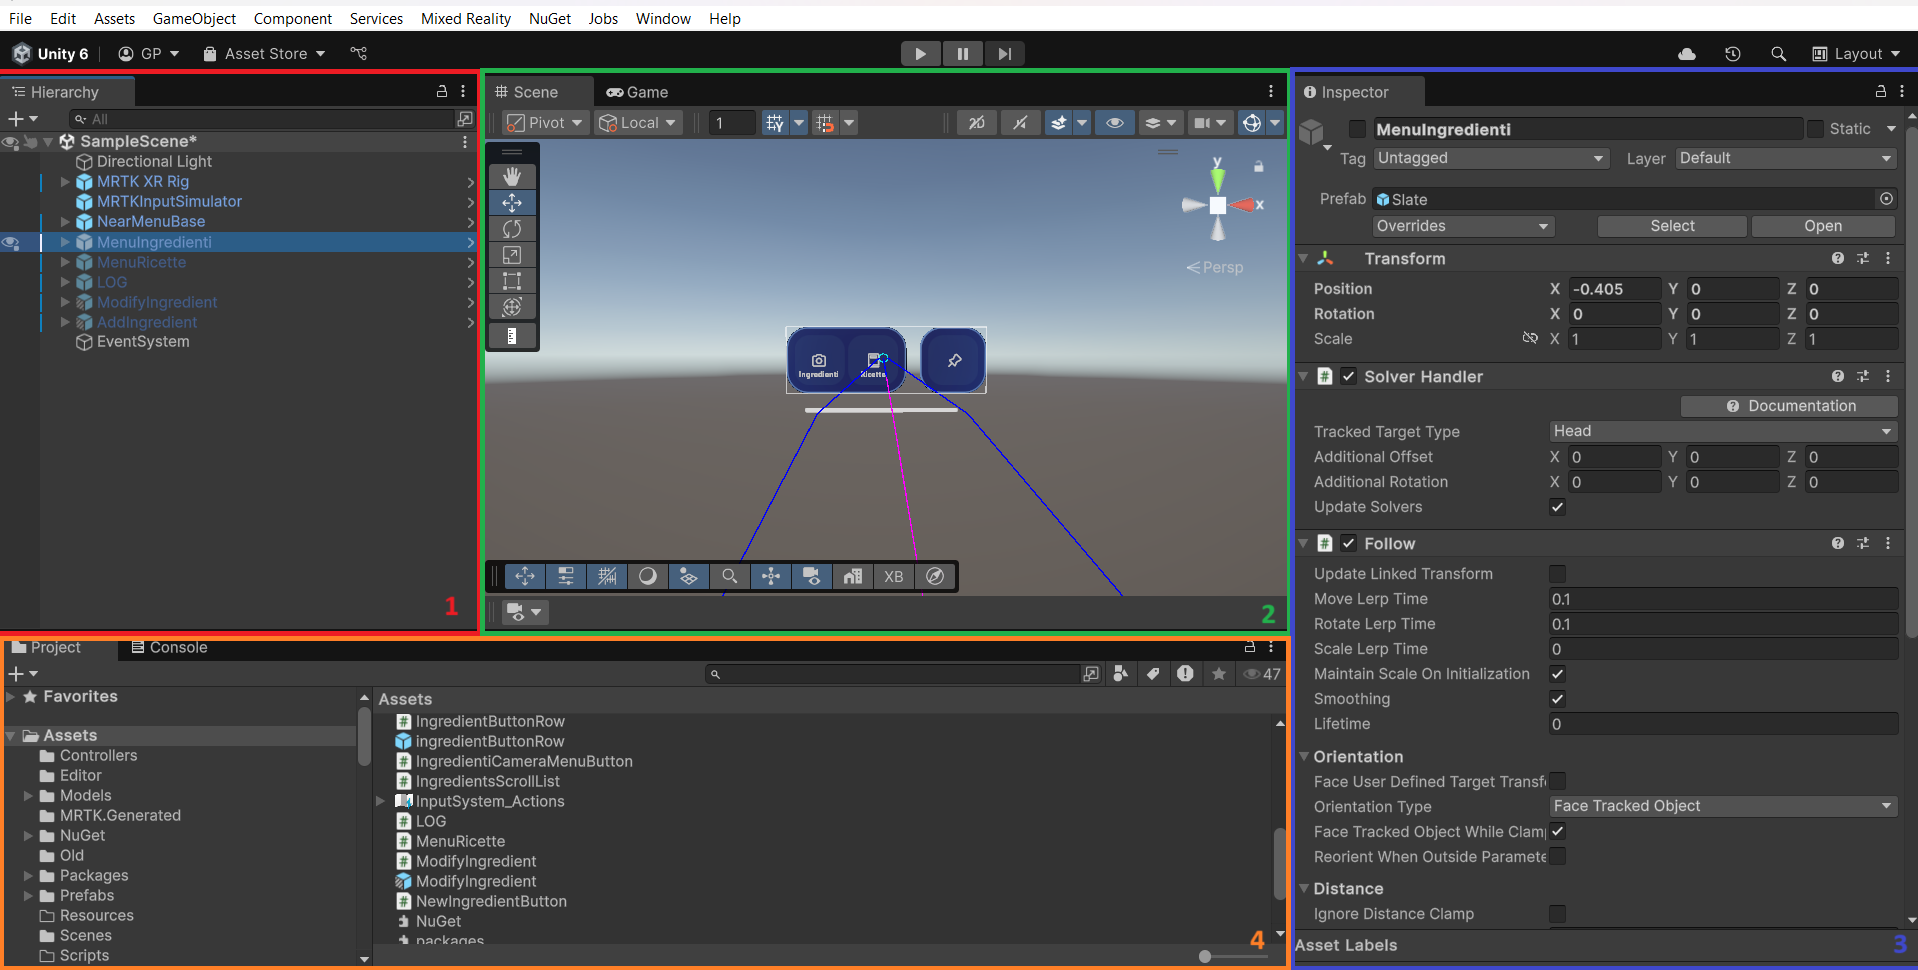
\includegraphics[width=\textwidth,height=\textheight,keepaspectratio]{figures/chapter_1/unityOverview.png}
\end{figure}
\begin{enumerate}
    \item \textbf{Gerarchia}: La gerarchia mostra tutti gli oggetti presenti nella scena. Puoi organizzare gli oggetti in una struttura ad albero, creando genitori e figli per raggruppare gli oggetti correlati.
    \item \textbf{Scena}: La scena è l'area di lavoro principale in Unity, dove puoi posizionare e organizzare gli oggetti 3D, le luci e le telecamere. Puoi visualizzare la scena in diverse modalità, come la vista 3D o la vista 2D.
    \item \textbf{Inspector}: L'Inspector mostra le proprietà e i componenti dell'oggetto selezionato nella gerarchia. Puoi modificare le proprietà degli oggetti, aggiungere componenti e configurare le impostazioni. Un componente potrebbe essere anche uno script C\# che definisce il comportamento dell'oggetto.
    \item \textbf{Project e Console}: La finestra Project mostra tutti i file e le risorse del tuo progetto, come modelli 3D, texture, suoni e script. Puoi organizzare le risorse in cartelle per una gestione più semplice. La Console mostra i messaggi di errore, avviso e debug generati durante l'esecuzione del gioco o dell'applicazione.
\end{enumerate}

\subsection{MRTK}
\begin{figure}[H]
    
\includegraphics[width=\textwidth,height=\textheight,keepaspectratio]{figures/chapter_1/logo_mrtk_unity_banner.png}
    \centering
\end{figure}
L'MRTK è un progetto della Microsoft che fornisce una serie di strumenti e librerie per lo sviluppo di applicazioni di realtà mista su piattaforme Microsoft, in particolare per gli HoloLens. Il toolkit include una serie di componenti e funzionalità per facilitare lo sviluppo di interfacce utente, il tracciamento delle mani, il riconoscimento vocale e altre funzionalità specifiche per la realtà mista. L'MRTK è progettato per essere facilmente integrato in Unity e offre una serie di esempi e documentazione per aiutare gli sviluppatori a iniziare rapidamente.\\
Oltre a supportare gli Hololens supporta anche altri visori come gli Oculus e permette anche di creare applicazioni AR (Argumented Reality) per Android e iOS.\cite{WhatIsMixedRealityToolkit}


\subsection{Google Gemini}
Google Gemini, inizialmente uscita sotto il nome di Google Bard, rappresenta uno dei più recenti sviluppi dell'intelligenza artificiale generativa di Google. Gemini, oltre a elaborare del testo, è in grado di comprendere anche immagini, audio, documenti e altri file di tipo testuale.
L'obiettivo di Google con Gemini è offrire un assistente personale basato su intelligenza artificiale che sia non solo utile e produttivo, ma anche creativo e capace di stimolare la curiosità dell'utente. In ambito produttivo, Gemini può ad esempio sintetizzare documenti lunghi, supportare attività di scrittura, aiutare nella programmazione e automatizzare attività complesse.\\
Nonostante il grande potenziale, Google riconosce che la tecnologia è ancora in una fase iniziale e presenta alcune limitazioni tipiche dei modelli linguistici di grandi dimensioni (LLM). Tra queste, vi sono il rischio di fornire risposte inaccurate, la possibilità che emergano bias nei contenuti generati, e la difficoltà nel rappresentare prospettive multiple su questioni soggettive. Inoltre, l'assistente può occasionalmente mostrare segnali di “personalizzazione” e sembrare esprimere emozioni o opinioni, che in realtà non possiede, essendo un modello statistico. Altri limiti includono i cosiddetti falsi positivi e falsi negativi, ossia casi in cui Gemini rifiuta di rispondere a domande appropriate o, al contrario, fornisce risposte inappropriate. Infine, il sistema può essere vulnerabile a prompt avversari, ovvero tentativi intenzionali di metterne alla prova i limiti o aggirarne i filtri di sicurezza.\\
Per evitare ciò, e rispettare le proprie linee guida, Google ha adottato un approccio responsabile nello sviluppo di Gemini, condudendo degli stress test svolti da team interni incaricati di individuare criticità, formando appositi "red team", composti da esperti e scienziati sociali.\cite{GeminiLaunch} \cite{GeminiAppOverview}

\chapter{Tecnologie concorrenti, simili e confronti}
\pagestyle{plain}

\section{Hardware}
Andiamo a esplorare altri Hardware concorrenti o simili agli Hololens 2, facendo un confronto delle caratteristiche principali e del perchè sono stati scartati per essere utilizzati in questo progetto.
\subsection{Meta Quest 3}
Il Meta quest 3 è il visore di punta sul mercato consumer di Meta, è un visore standalone, ma che si può collegare anche al PC, con un sistema operativo basato su Android chiamato Meta Horizon OS. A differenza degli Hololens 2 ha un processore molto più potente, uno Snapdragon XR2 Gen2, con al massimo 512GB di memoria interna e 8Gb di Ram. A differenza degli Hololens2 ha uno schermo LCD con una risoluzione di 2064x2208 per occhio, e un refresh rate massimo di 120Hz. Dato che ha un display la realtà mista viene garantita tramite un sistema di passthrough, che permette di vedere il mondo reale attraverso le telecamere del visore, che riescono a ricostruire in maniera quasi perfetta la normale visione di un occhio umano. Dal punto di vista dello sviluppo di app questo avviene sempre con Unity e un pacchetto di sviluppo, ma a differenza degli Hololens 2 non è possibile accedere in nessun modo alle fotocamere frontali, diminuendo di molto le capacità delle applicazioni in realtà mista.
\subsection{HoloLens 1}
Gli Hololens di prima generazione, usciti nel 2016, sono i predecessori degli Hololens 2, sono dotati di un Intel Atom x5-Z8100, 2Gb di RAM e 64Gb di memoria interna, le prestazioni, comparate con quelle del visore di nuova generazione, sono nettamente inferiori, inoltre questo visore è in fase di dismissione, in favore della nuova generazione. Quindi la scelta degli Hololens 2 è abbastanza banale, anche solo per il confronto di prestazioni.

\section{Tecnologie di Visualizzazione}
Oltre alla MR (Mixed Reality) esistono altre tecnologie di visualizzazione, le più importanti sono la VR (Virtual Reality) e la AR (Augmented Reality).
\subsection{Realtà Virtuale (VR) }
La Realtà Virtuale crea un ambiente virtuale completamente immmersivo dove l'utente può muoversi e interagire, ad esempio prendendo oggetti. Ogni utente può avere anche un avatar e interagire con altri utenti nel mondo virtuale. Di solito questo tipo di tecnologia viene utilizzata con dei visori dotati di schermi che coprono completamente il campo visivo dell'utente, e che sono dotati di sensori di movimento, per permettere all'utente di muoversi in questo mondo virtuale. La VR viene utilizzata principalmente per videogiochi, ma anche per applicazioni professionali, come ad esempio la simulazione di ambienti per la formazione, ma anche per la creazione di riunioni aziendali virtuali.

\subsection{Realtà Aumentata (AR) }
Il più famoso esempio di Realtà Aumentata potrebbe essere il gioco Pokemon Go, dove gli utenti possono vedere i Pokemon nel mondo reale attraverso lo schermo del proprio smartphone per poi catturarli. La AR permette di sovrapporre oggetti virtuali al mondo reale, visualizzando informazioni extra come testi, indicazioni stradali, e oggetti 3d, ma non permette di interagire con essi.

\subsection{Differenze e confronto tra AR e MR}
La Realtà Aumentata e la Realtà Mista sono due tecnologie simili, ma con differenze fondamentali. La Realtà Aumentata sovrappone oggetti virtuali al mondo reale, ma non permette di interagire con essi in modo significativo. La Realtà Mista, invece, integra gli oggetti virtuali nel mondo reale in modo più profondo, permettendo all'utente di interagire con essi come se fossero parte del mondo reale. Ad esempio, in un'applicazione di Realtà Mista, un utente potrebbe afferrare un oggetto virtuale e spostarlo virtualmente nello spazio reale, mentre in un'applicazione di Realtà Aumentata l'oggetto virtuale rimarrebbe statico e non interagirebbe con l'ambiente circostante.

\subsection{Differenze e confronto tra VR e MR}
La Realtà Virtuale e la Realtà Mista sono due tecnologie che offrono esperienze immersive, ma con differenze significative. La Realtà Virtuale crea un ambiente completamente virtuale, isolando l'utente dal mondo reale, mentre la Realtà Mista integra elementi virtuali nel mondo reale, consentendo interazioni più naturali e intuitive per l'utente.

\cite{DifferenceMeta-AR-VR-MR} \cite{DifferenceIBM-AR-VR-MR}
\chapter{Processo e tecniche di sviluppo per applicazioni MR per Hololens2}
\pagestyle{plain}
In questa sezione andremo a vedere come inizializzare un progetto Unity e utilizzare l'MRTK al suo interno. Successivamete si andrà ad approfondire entrambi, andando a vedere il funzionamento dei componenti utilizzati in questo progetto e le tecniche di programmazione utilizzate. 


\section{Setup di Unity}
\subsection{Installazione di Unity}
Andare nel sito ufficiale di Unity e scaricare l'ultima versione disponibile. Dopo l'installazione ci si troverà davanti all'Unity Hub, qui la schermata potrebbe leggermente cambiare a seconda della versione ma delle opzioni 3d disponibili \textbf{non} bisogna scegliere la versione \textbf{URP} o \textbf{HDRP} ma la versione normale \textbf{3D}. 
\begin{figure}[H]
    \centering
    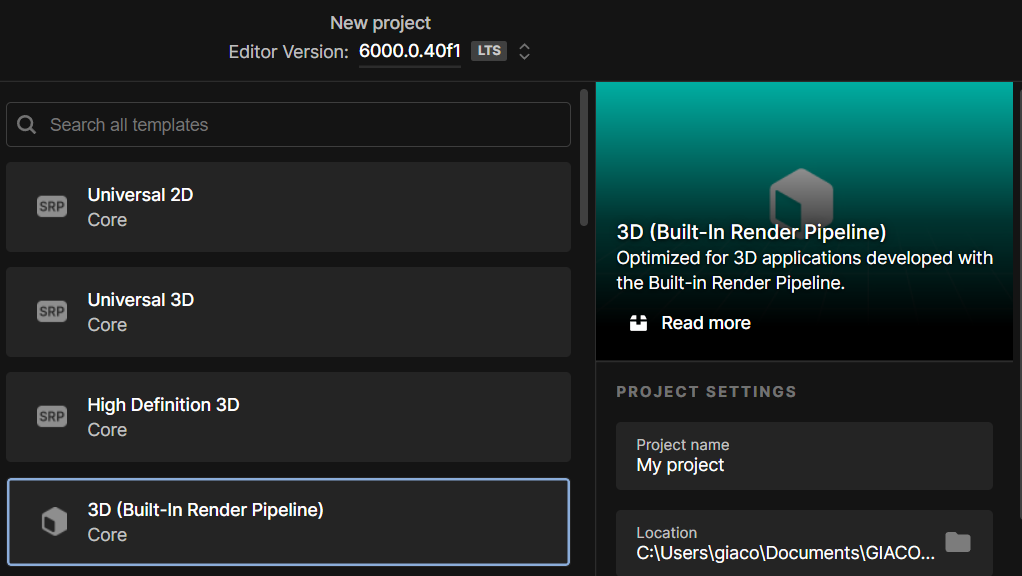
\includegraphics[width=0.9\textwidth,height=\textheight,keepaspectratio]{figures/chapter_1/unityHub.png}
    \caption{In questo caso la versione corretta è quella selezionata}
\end{figure}
Dopo aver dato nome al progetto e selezionata la cartella di installazione andiamo subito a modificare le impostazioni di build.
\begin{figure}[H]
    \centering
    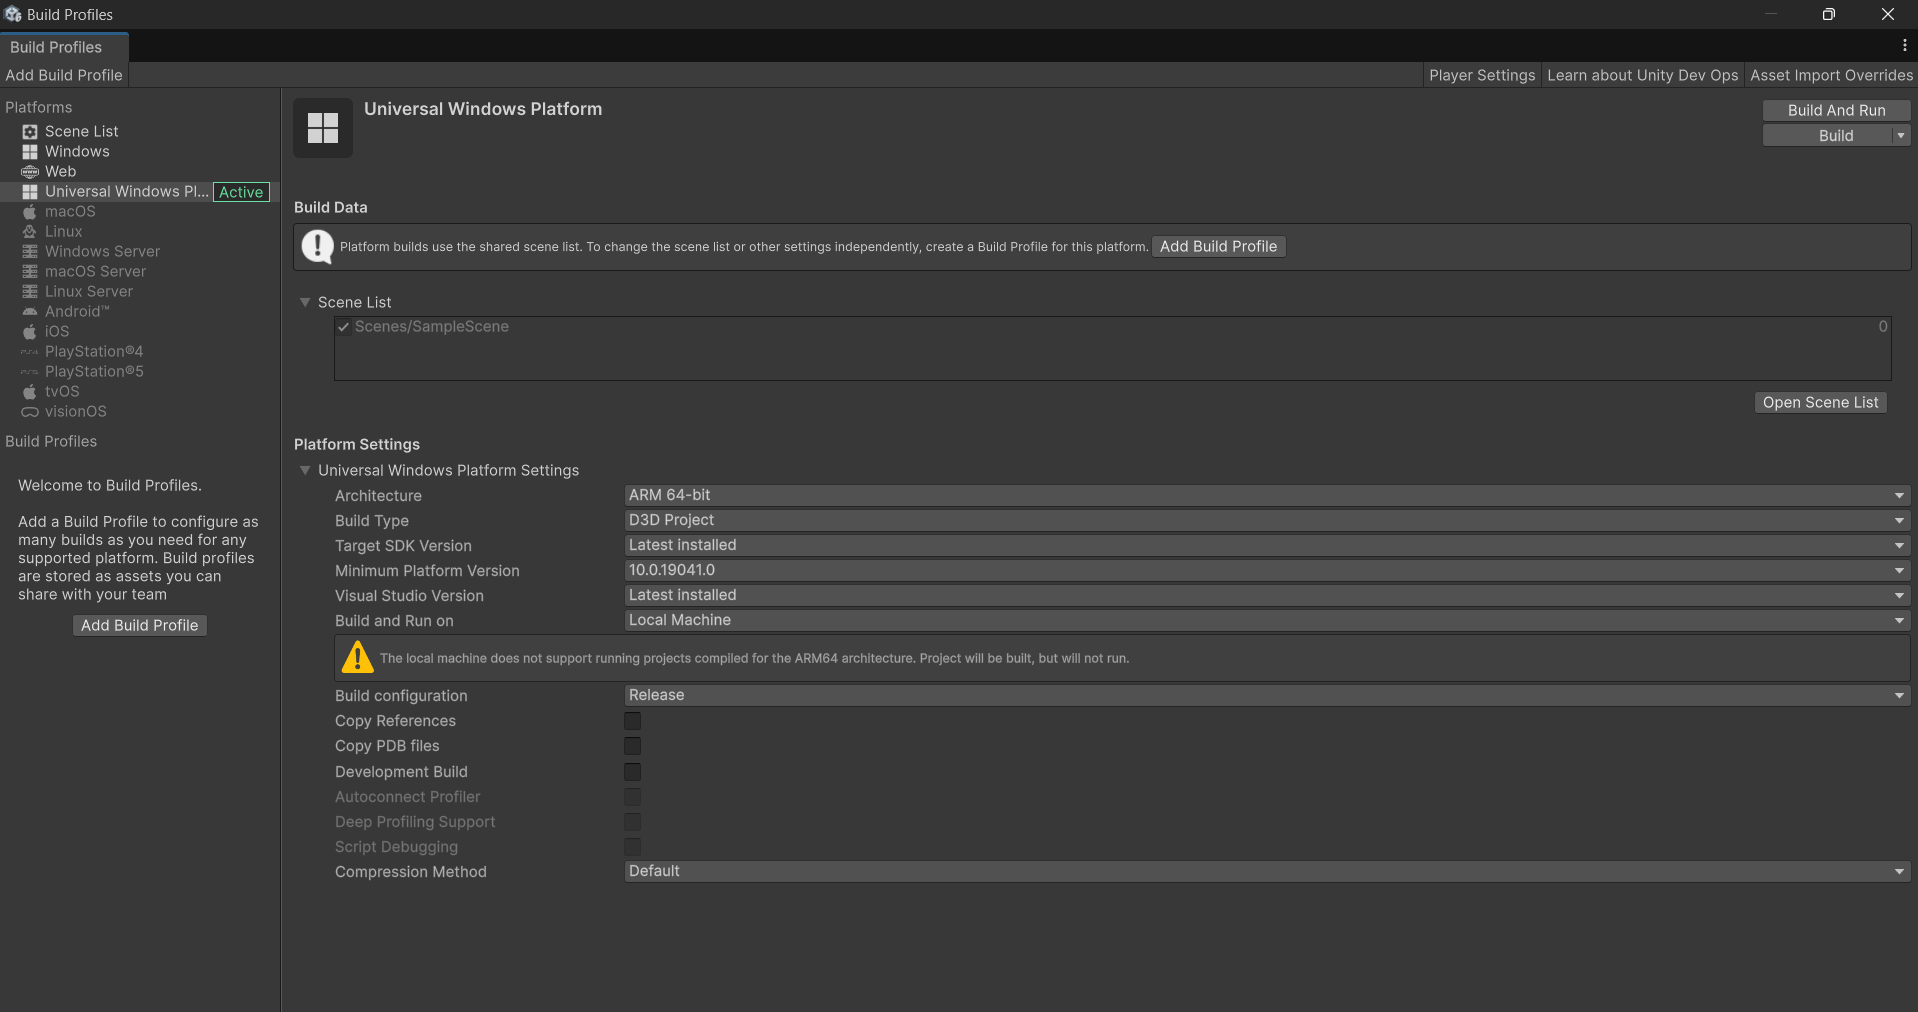
\includegraphics[width=0.9\textwidth,height=\textheight,keepaspectratio]{figures/chapter_1/impostazioniBuild.png}
    \caption{Da notare il "Build Type"}
\end{figure}
Prima di tutto bisogna essere sicuri di aver attivato la build per l'Universal Windows Platform e di aver selezionato la piattaforma \textbf{ARM64} come architettura, questo è fondamentale per il corretto funzionamento dell'applicazione su Hololens2, poi bisogna essere sicuri di avere come build type \textbf{D3D}.
\subsection{Installazione di Mixed Reality Feature Tool}
Dopo questi passaggi scaricare il "Mixed Reality Feature Tool" dal sito ufficiale di Microsoft, questo strumento ci permette di scaricare e installare l'MRTK (Mixed Reality Toolkit) direttamente all'interno del nostro progetto. Una volta scaricato, aprire l'eseguibile, selezionare il path del progetto Unity, nella schermata successiva selezionare tutta la sezione "MRTK3" e alla sezione "Platform Support" selezionare "Mixed Reality OpenXR Plugin". 
\begin{figure}[H]
    \centering
    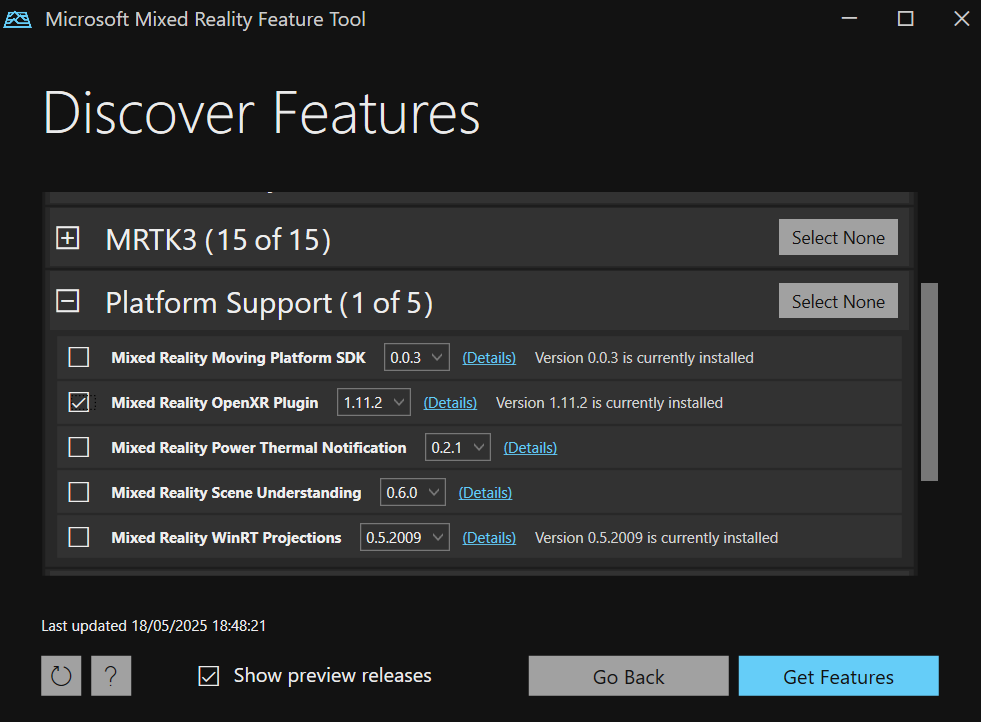
\includegraphics[width=0.9\textwidth,height=\textheight,keepaspectratio]{figures/chapter_1/mixedRealityTool.png}
    \caption{}
\end{figure}
Dopo ciò ritornare su Unity e aspettare che il pacchetto venga importato.
\subsection{Impostazioni del progetto e della scena}
 Una volta completata l'installazione dei pacchetti andare nelle impostazione del progetto e seguire le seguenti immagini:
\begin{figure}[H]
    \centering
    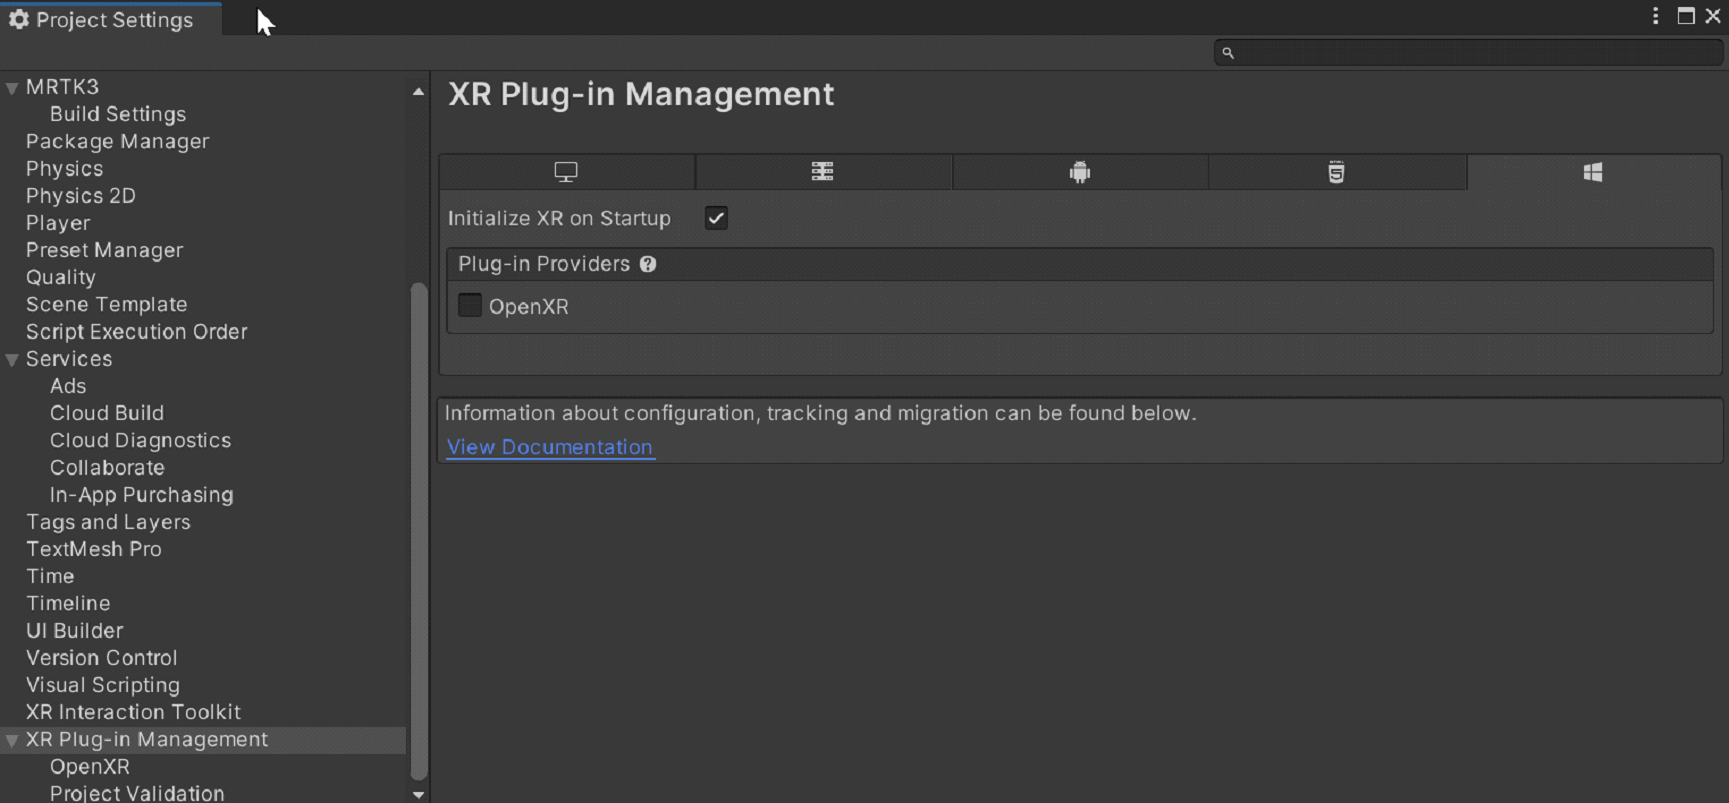
\includegraphics[width=0.9\textwidth,height=\textheight,keepaspectratio]{figures/chapter_1/projectSetting1.png}
    \caption{Andare nelle impostazioni del progetto e selezionare la sezione "XR Plug-in Management"}
\end{figure}
\begin{figure}[H]
    \centering
    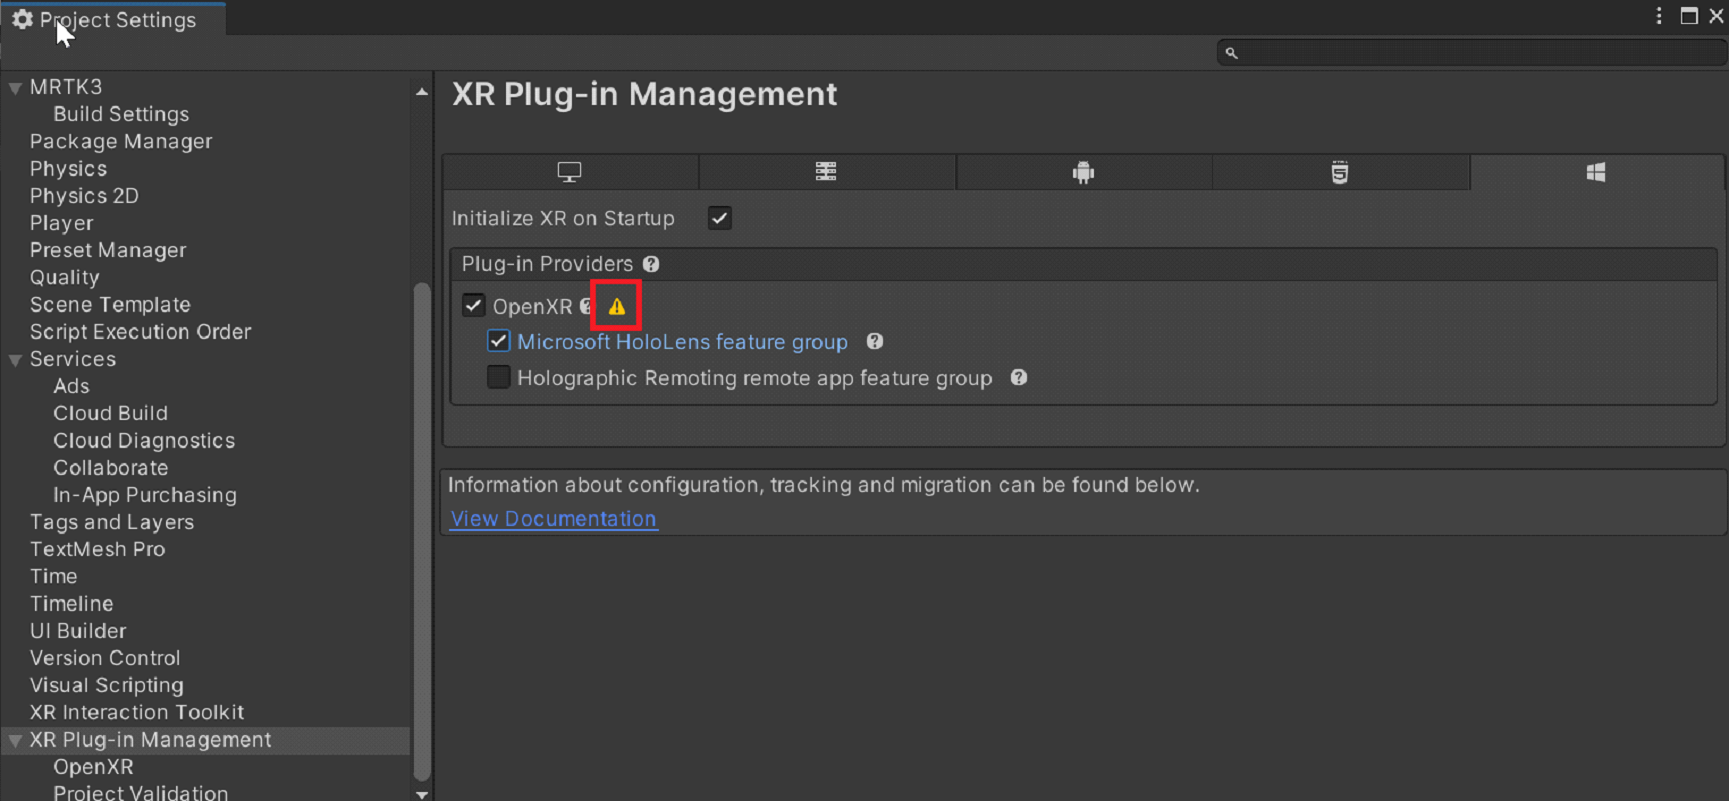
\includegraphics[width=0.9\textwidth,height=\textheight,keepaspectratio]{figures/chapter_1/projectSetting2.png}
    \caption{Abilitare l'OpenXR}
\end{figure}
\begin{figure}[H]
    \centering
    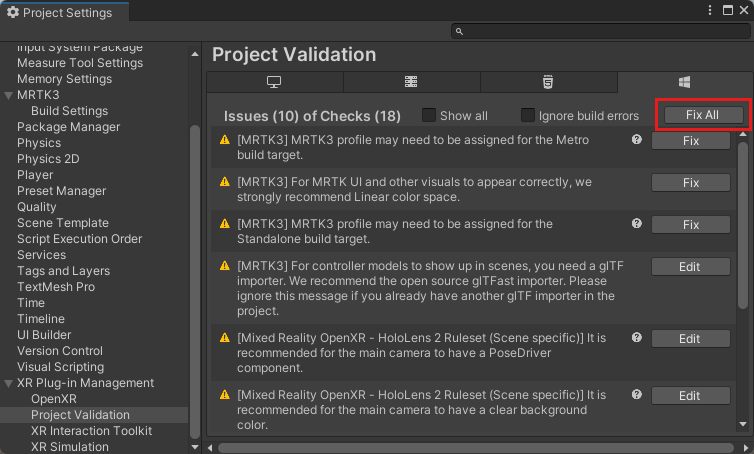
\includegraphics[width=0.9\textwidth,height=\textheight,keepaspectratio]{figures/chapter_1/projectSetting3.png}
    \caption{Se compare il triangolo giallo, cliccarci sopra e premere "Fix All"}
\end{figure}
\begin{figure}[H]
    \centering
    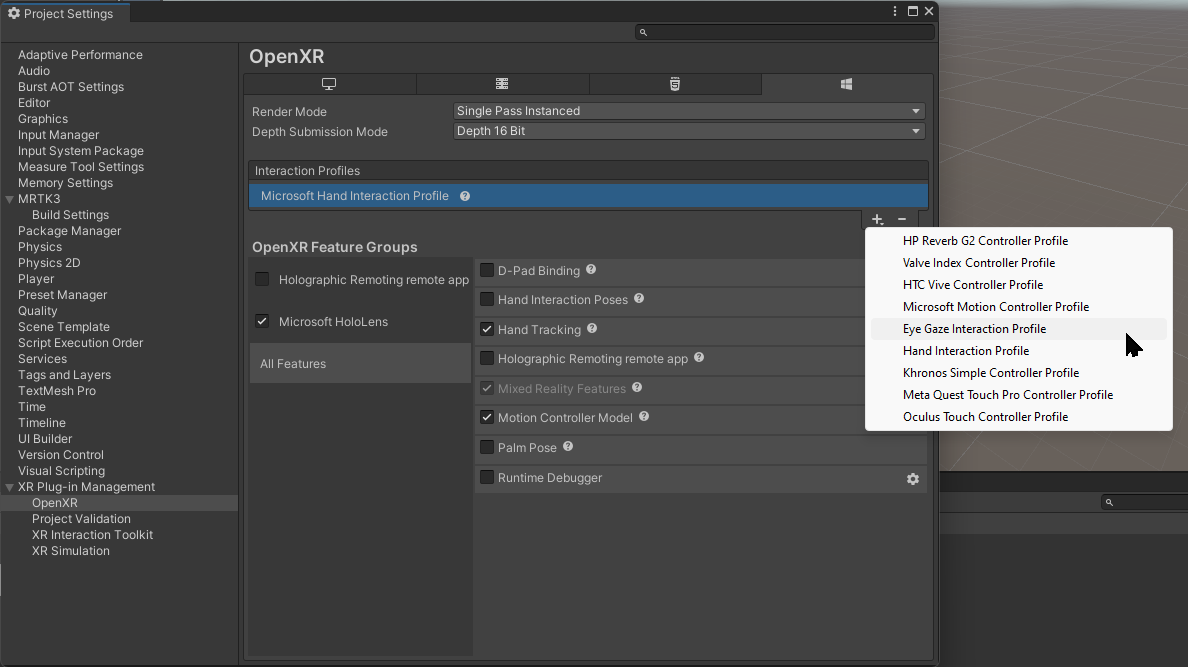
\includegraphics[width=0.9\textwidth,height=\textheight,keepaspectratio]{figures/chapter_1/projectSetting4.png}
    \caption{Inserire i seguenti profili e abilitare le spunte in foto}
\end{figure}
\begin{figure}[H]
    \centering
    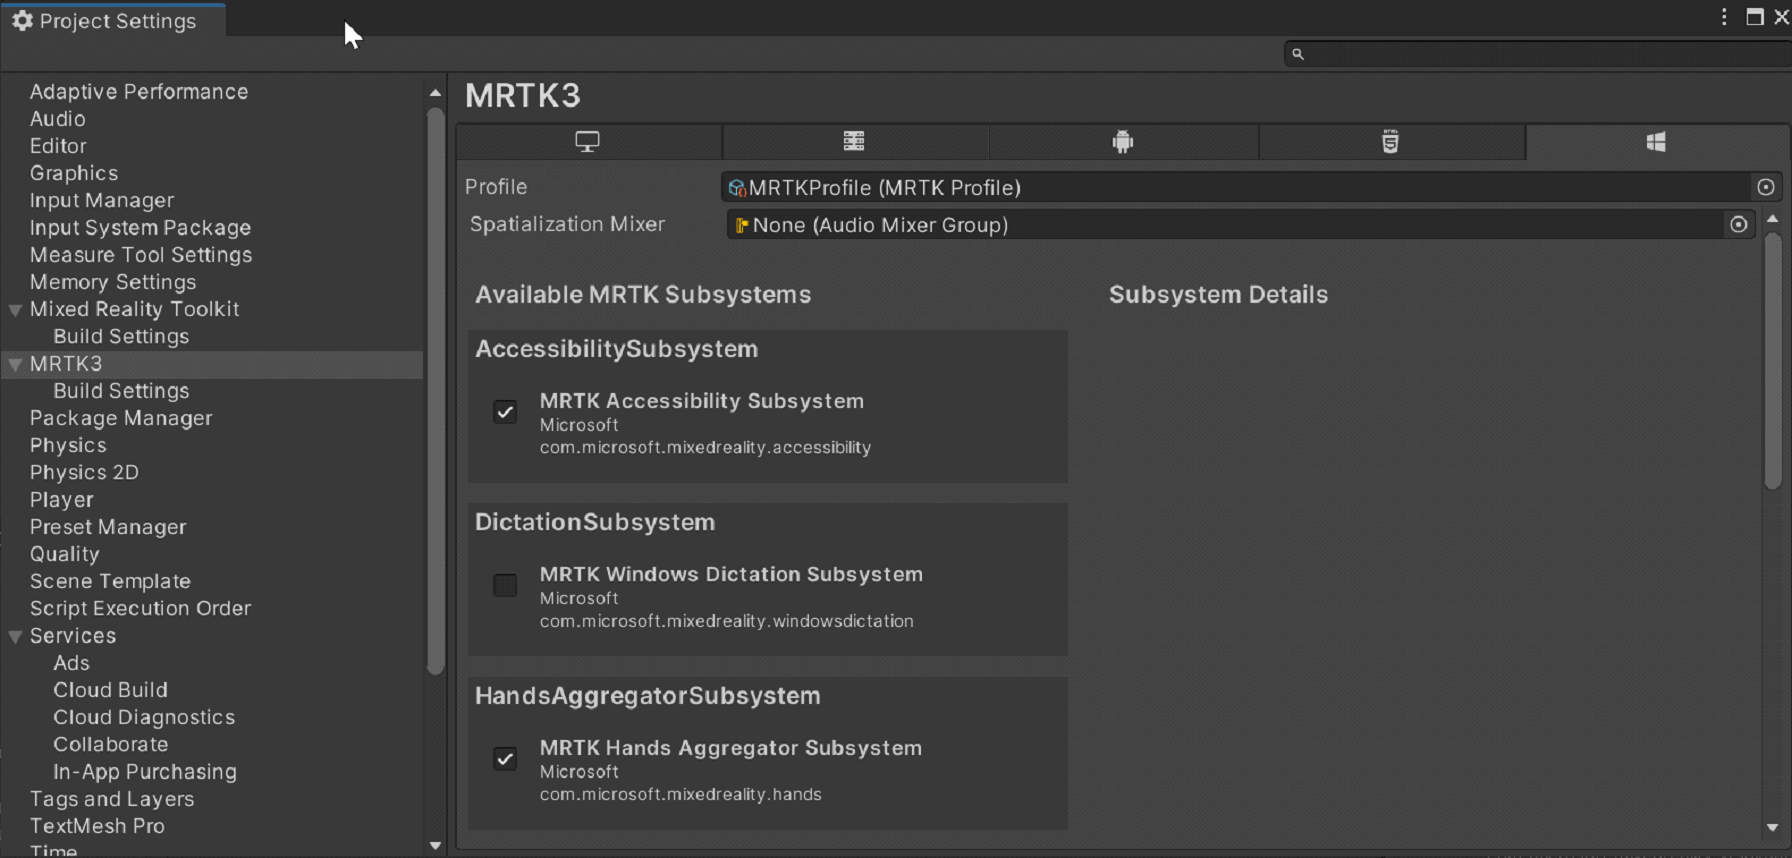
\includegraphics[width=0.9\textwidth,height=\textheight,keepaspectratio]{figures/chapter_1/projectSetting5.png}
    \caption{Nella sezione MRTK3 selezionare il profilo come in figura}
\end{figure}
Una volta completati questi passaggi tornare alla scena principale di Unity, andare nella sezione che mostra le gerarchia degli oggetti ed eliminare tutto, poi andare nella sezione in basso denominata "Project", navigare dentro "Pakages" -> "MRTK Input" -> "Assets" -> "Prefabs", trovare "MRTK XR Rig" e trascinarlo nella scena.
\begin{figure}[H]
    \centering
    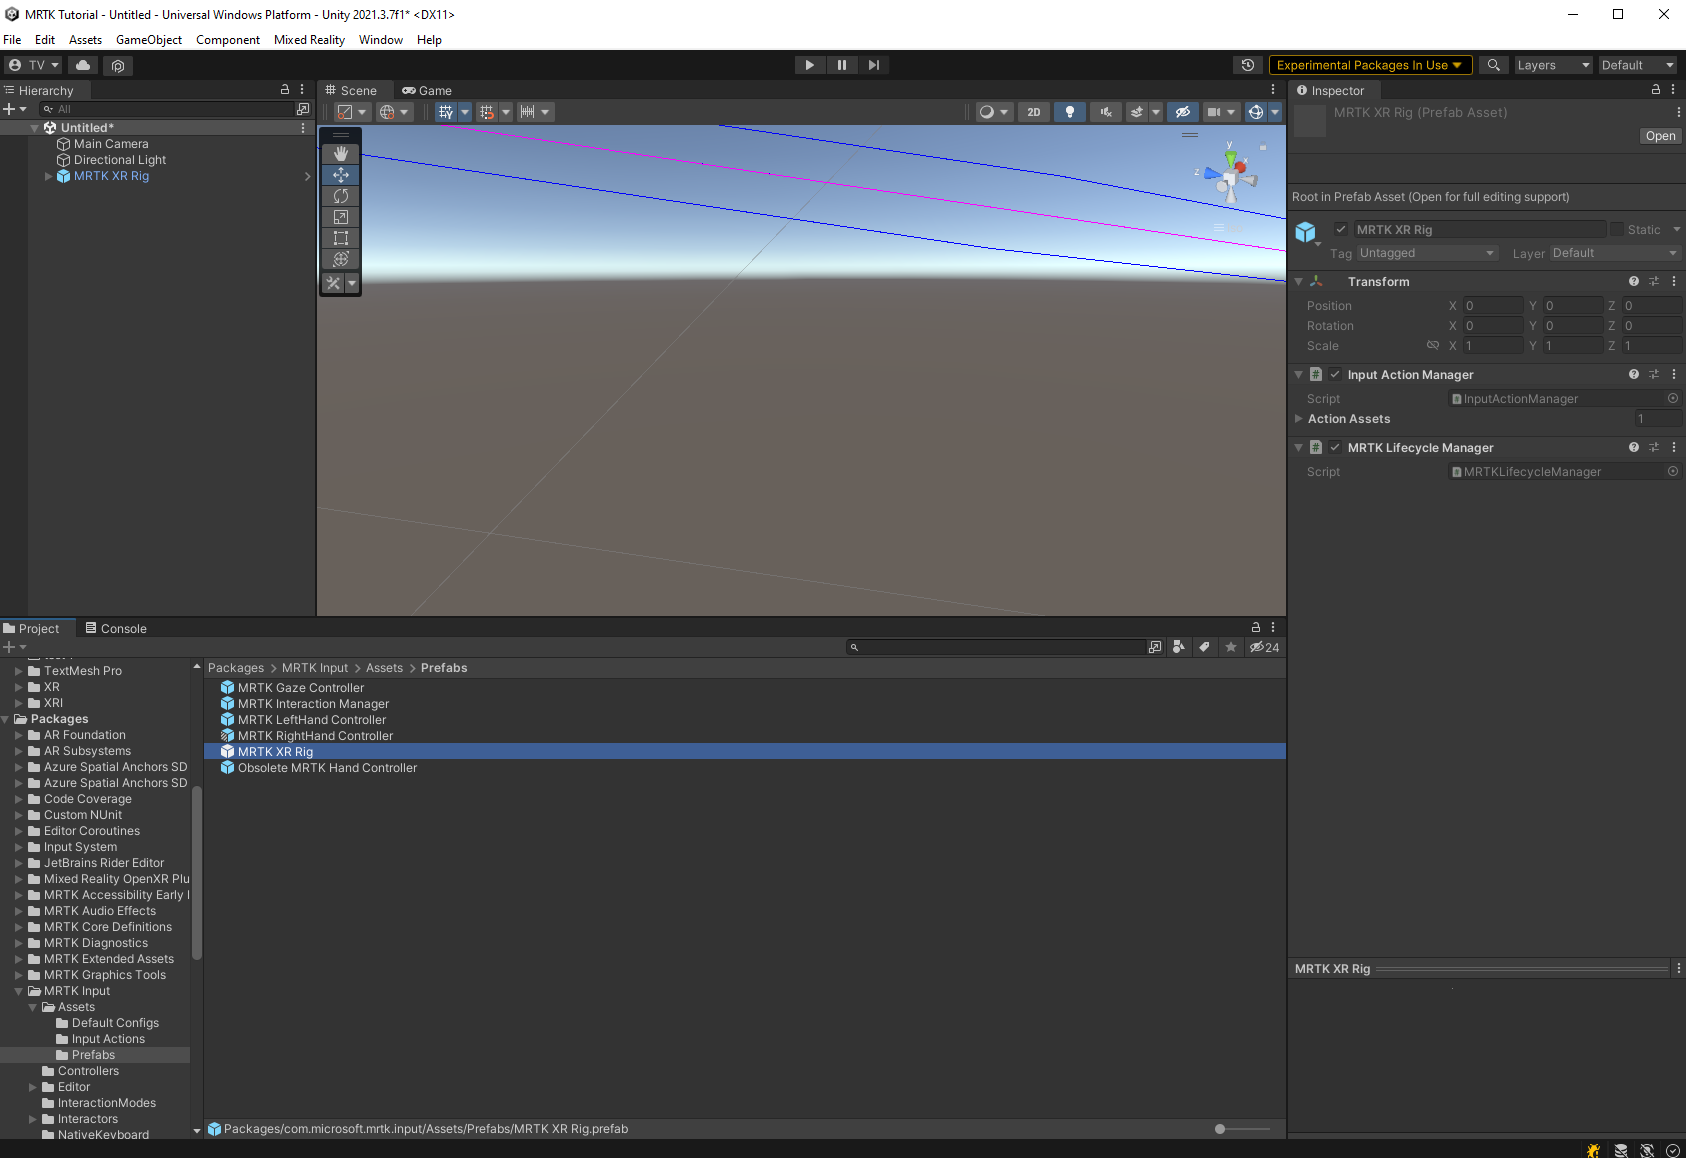
\includegraphics[width=0.9\textwidth,height=\textheight,keepaspectratio]{figures/chapter_1/mrtk-xr-rig-prefab.png}
    \caption{}
\end{figure}
Fare la stessa cosa con "MRTK Input Simulator" che si trova in "Packages" -> "MRTK Input" -> "Simulation" -> "Prefabs".
Con questo il setup di Unity è completo, ora possiamo iniziare a lavorare con l'MRTK e a sviluppare la nostra applicazione.
\section{MRTK3.0}
Andiamo a vedere i principali componenti utilizzati in questo progetto e il loro funzionamento.
\subsection{Tabs}
Questo componente è stato utilizzato per visualizzare le tre ricette generate da Gemini e, nella Slate principale, per separare la foto scattata dalla lista di ingredienti rilevati dall'AI.

\begin{figure}[H]
    \centering
    
\includegraphics[width=0.5\textwidth,height=\textheight,keepaspectratio]{figures/chapter_1/tabs1.png}
    \caption{Tabs nel menu della fotocamera e ingredienti}
\end{figure}

\begin{figure}[H]
    \centering
    
\includegraphics[width=0.5\textwidth,height=\textheight,keepaspectratio]{figures/chapter_1/tabs2.png}
    \caption{Tabs nel menu delle ricette}
\end{figure}
Per creare un menu di Tabs dobbiamo avere due o più bottoni e dei relativi contenuti che verranno nascosti e mostrati a seconda del tab selezionato.
\begin{figure}[H]
    \centering
    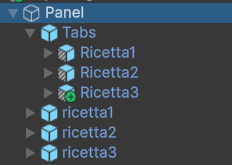
\includegraphics[width=0.4\textwidth,height=\textheight,keepaspectratio]{figures/chapter_1/tabs-gerarchia.png}
    \caption{Gerarchia dei oggetti}
\end{figure}

Gli elementi denominati "Ricetta1", "Ricetta2" e "Ricetta3" sono i bottoni che rappresentano le singole tab, mentre "ricetta1", "ricetta2" e "ricetta3" sono i contenuti che verranno mostrati quando si seleziona il rispettivo tab. Per fare ciò dobbiamo avere il seguente componente nel GameObject Tabs:

\begin{figure}[H]
    \centering
    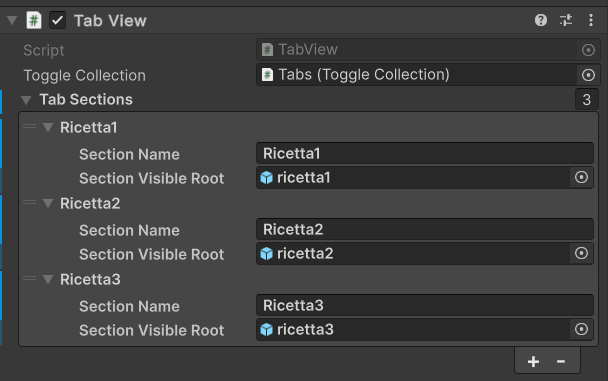
\includegraphics[width=0.4\textwidth,height=\textheight,keepaspectratio]{figures/chapter_1/componente-tabs.png}
    \caption{Componente per il funzionamento delle tabs}
\end{figure}

 In "Toggle Collection" andiamo a trascinare il GameObject padre "Tabs", collezione dei tre bottoni, e in "Tab Selections" andiamo a impostare gli oggetti da visualizzare quando si premono i bottoni. Da notare che l'ordine in cui abbiamo messo i bottoni nel padre "Tabs" è lo stesso ordine in cui andremo a mettere gli oggetti da visualizzare nel componente, quindi il primo bottone mostrerà il primo oggetto e così via. \cite{MRTKtabs}

\subsection{Scroll list}
La scroll list utilizzata in questo progetto è un prefab che si trova all'interno dei pakages dell'MRTK3, precisamente in "MRTK UX Components" -> "Experimental" -> "Scrollable". Se apriamo il prefab la gerarchia di GameObject è la seguente:

\begin{figure}[H]
    \centering
    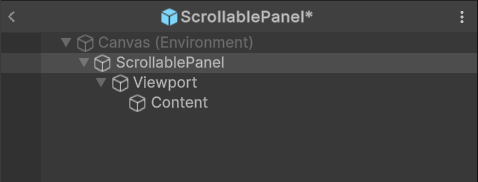
\includegraphics[width=0.4\textwidth,height=\textheight,keepaspectratio]{figures/chapter_1/GerarchiascrollPanel.png}
    \caption{Gerarchia del prefab ScrollablePanel}
    \label{fig:scrollablePanel}
\end{figure}

In Content andiamo a mettere gli oggetti che vogliamo visualizzare e scorrere, Viewport, con i suoi componenti, ci permette di visualizzare solo una parte del contenuto se questo è più grande della finestra di visualizzazione, mentre nell'oggetto ScrollablePanel c'è il componente che ci permette di scorrere il contenuto e definisce la scroll list. 
\begin{itemize}
    \item \textbf{Content}: è consigliabile che abbia un componente come un Grid Layout Group o un Vertical Layout Group, in modo da avere una disposizione ordinata degli oggetti al suo interno.
    \item \textbf{Viewport}: è l'oggetto che contiene il contenuto visibile della scroll list, quindi è fondamentale che abbia un componente Rect Mask 2D, in modo da mascherare il contenuto che esce dalla finestra di visualizzazione.
    \item \textbf{Scrollable Panel}: è l'oggetto che contiene il componente Scroll Rect, a cui dobbiamo assegnare il viewport e le due barre di scorrimento se presenti. In questo modo possiamo scorrere il contenuto all'interno della finestra di visualizzazione. Oltre ad altri componenti c'è anche "Scrollable", dove dobbiamo impostare la "Scroll Rect" ed è un componente dell'MRTK3
\end{itemize}

\begin{figure}[H]
    \centering
    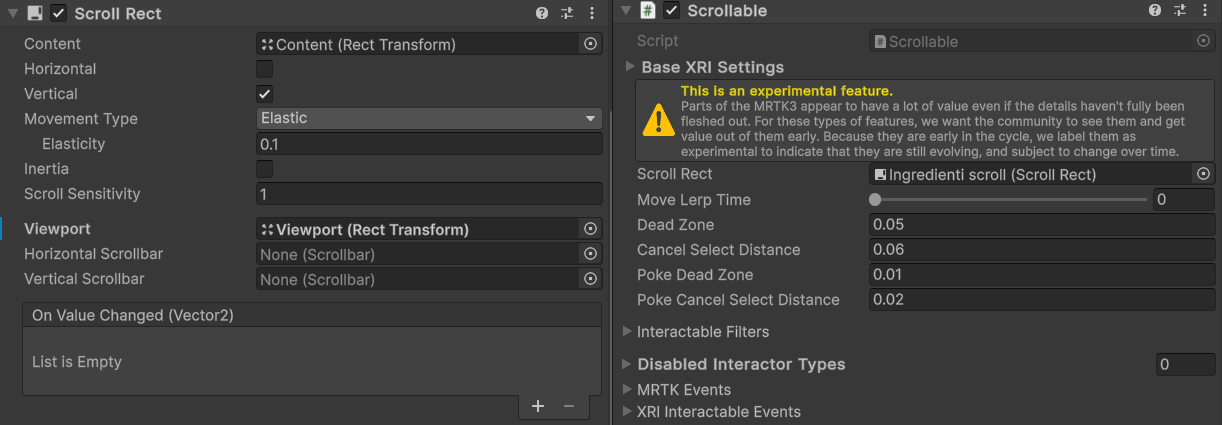
\includegraphics[width=0.8\textwidth,height=\textheight,keepaspectratio]{figures/chapter_1/ComponentiScrollBar.png}
    \caption{Componenti per \textbf{Scrollable Panel}}
\end{figure}

\subsection{Slate}
La Slate offre una finestra che consente la visualizzazione di contenuti 2D, come testo, immagini e elementi grafici come bottoni e menu, come una vera e propria finestra di una applicazione desktop. La Slate è un oggetto prefab che si trova all'interno dei pakages dell'MRTK3, precisamente in "MRTK UX Components (Non-Canvas)" -> "Slates".

\begin{figure}[H]
    \centering
    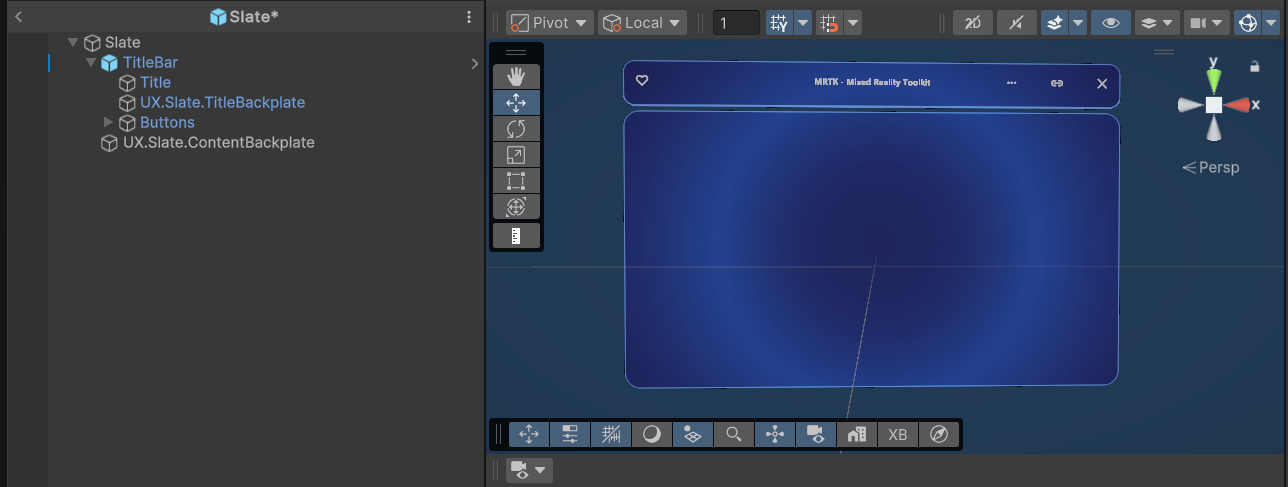
\includegraphics[width=0.8\textwidth,height=\textheight,keepaspectratio]{figures/chapter_1/slate.png}
    \caption{Gerarchia e UI della Slate}
\end{figure}

La Slate è composta principalmente da:
\begin{itemize}
    \item \textbf{TitleBar}: è la barra in alto, ha due bottoni personalizzabili, altri due bottoni per chiudere la finestra e abilitare il follow e il titolo.
    \item \textbf{UX.Slate.ContentBackplate}: il contenitore padre dove andremo a mettere gli oggetti che vogliamo visualizzare all'interno della finestra
\end{itemize}

La Slate può essere trascinata dove si vuole prendendola dalla TitleBar, può essere chiusa e si può abilitare il follow, in modo che segua la posizione dell'utente.
\cite{MRTKslate}

\subsection{Near Menu}
Il Near Menu offre un menù che può essere spostato o può seguire l'utente, in modo tale da non dare fastidio alle interazioni con gli altri elementi. Il Near Menu lo possiamo trovare sotto forma di Prefab all'interno dei pakages dell'MRTK3, precisamente in "MRTK UX Components" -> "Near Menu".

\begin{figure}[H]
    \centering
    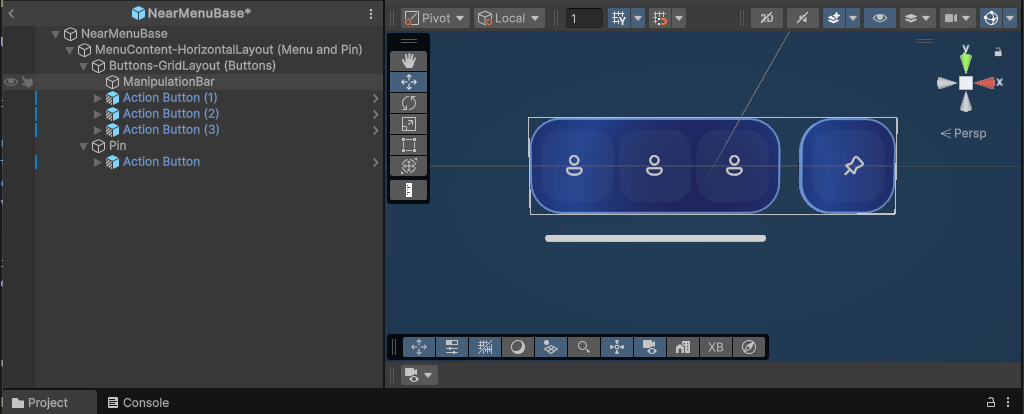
\includegraphics[width=0.8\textwidth,height=\textheight,keepaspectratio]{figures/chapter_1/nearMenu.png}
    \caption{Gerarchia e UI del Near Menu}
\end{figure}

Il Near Menu è composto principalmente da:
\begin{itemize}
    \item \textbf{Bottoni}: Si trovano all'interno di un Grid Layout e ne possiamo aggiungere quanti vogliamo, anche creando più righe e colonne.
    \item \textbf{PinButton}: è il bottone che permette di fissare il menù nella posizione in cui si trova, disattivando il follow
    \item \textbf{ManipulatorBar}: è la barra bianca in basso che permette di prendere e spostare il menù
\end{itemize}

Comportamenti principali del Near Menu:
\begin{itemize}
    \item \textbf{Tag-along}: il menù segue l'utente ponendosi ad una distanza di 30-60cm 
    \item \textbf{Pin}: usando il bottone del pin, situato nella parte più a destra, si fissa il menù nella posizione in cui si trova e si disattiva il follow
    \item \textbf{Grab and move}: essendo il menù un oggetto prendibile e spostabile, si può riposizionare in qualsiasi punto dello spazio prendendolo dalla barra bianca in basso
\end{itemize}

\cite{MRTKnearMenu}

\section{Programmazione in Unity con C\#}
\subsection{MonoBehaviour}
\begin{wrapfigure}{r}{0.50\textwidth} %this figure will be at the right
    \centering
    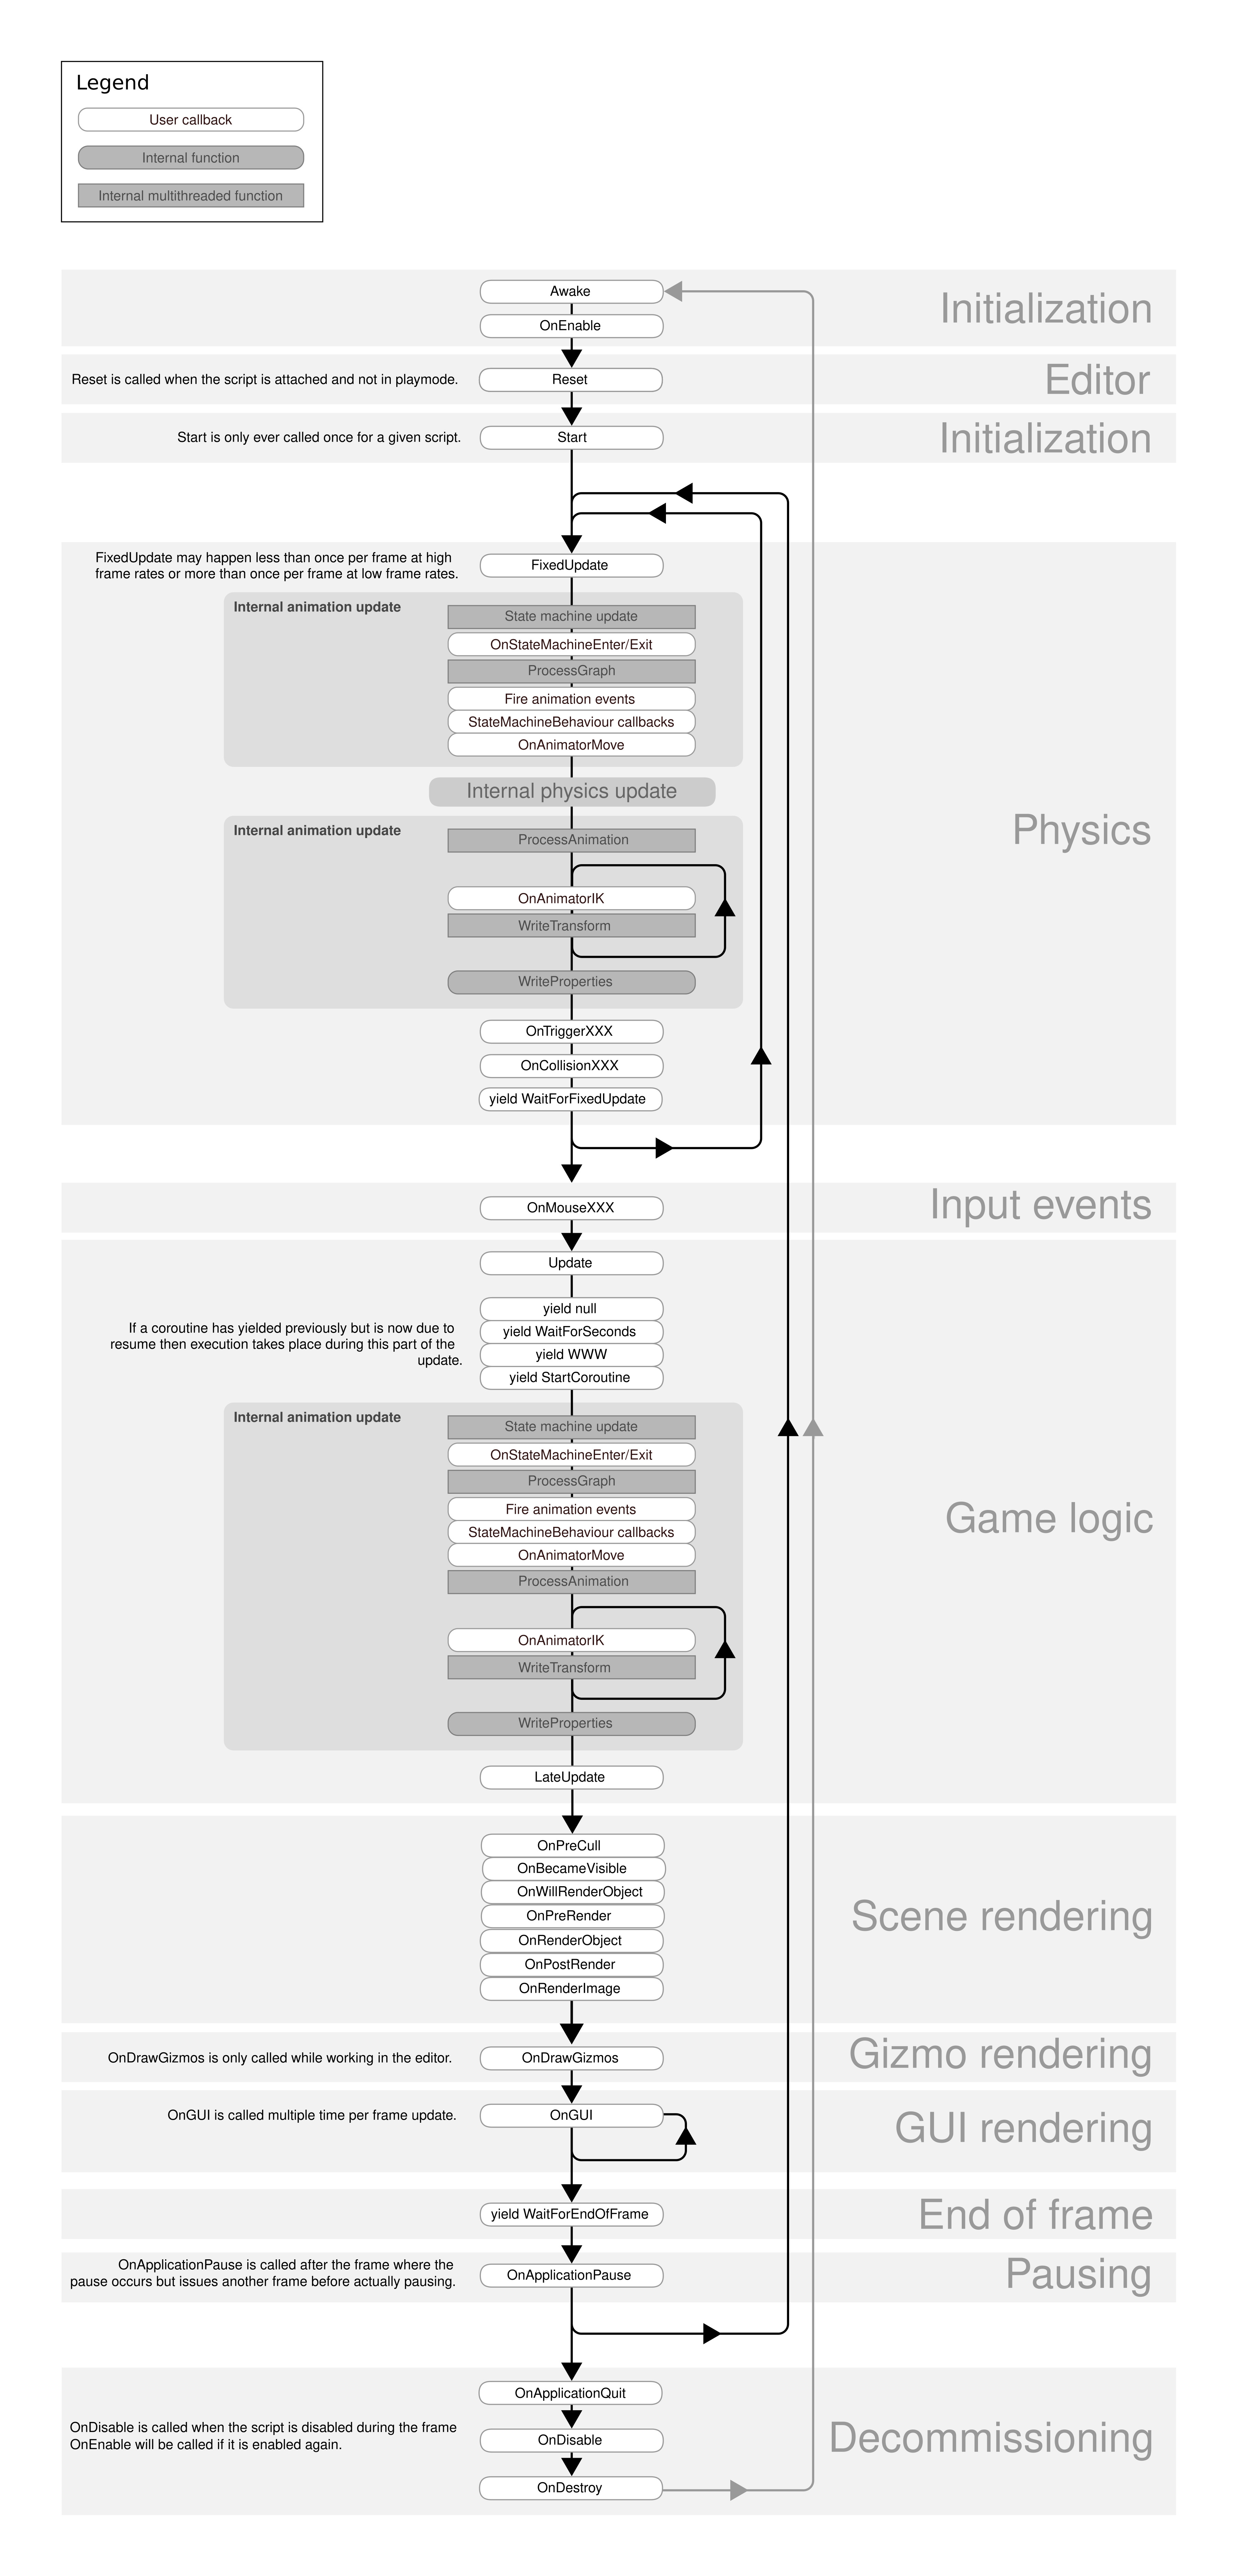
\includegraphics[width=0.40\textwidth]{figures/chapter_1/monobehaviour_flowchart.jpg}
\end{wrapfigure}
Il MonoBehaviour è la classe base da cui derivano tutti gli script in Unity. Quando creiamo uno script in Unity, automaticamente ereditiamo da MonoBehaviour, il che ci permette di utilizzare i metodi e le proprietà che Unity mette a disposizione per gestire il ciclo di vita degli oggetti della scena.
\cite{MonoBehaviour} 

I metodi principali utilizzati nel progetto sono:
\begin{itemize}
    \item \textbf{Awake}: viene chiamato prima di Start quando il GameObject padre è attivo e si inizializza al caricamento della scena o passa da uno stato disattivo ad attivo \cite{AwakeMonoBehaviour}
    \item \textbf{OnEnable}: viene chiamato quando l'oggetto viene abilitato e diventa attivo \cite{OnEnableMonoBehaviour}
    \item \textbf{Start}: viene chiamato una sola volta all'inizio del ciclo di vita dello script, utile per inizializzare variabili o impostare lo stato iniziale dell'oggetto \cite{StartMonoBehaviour}
    \item \textbf{Update}: viene chiamato una volta per frame, ed è il metodo principale per gestire la logica del GameObject \cite{UpdateMonoBehaviour}
    \item \textbf{OnDisable}: viene chiamato quando l'oggetto viene disabilitato \cite{OnDisableMonoBehaviour}
\end{itemize}

\subsection{Prefab}
\label{sec:prefab}
I Prefab consentono di configurare e creare un GameObject con tutti i suoi componenti e proprietà, così da riutilizzarlo e istanziarlo nella scena quante volte si vuole senza doverlo ricreare da capo ogni volta.
\begin{figure}[H]
    \centering
    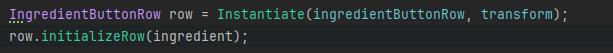
\includegraphics[width=0.8\textwidth,height=\textheight,keepaspectratio]{figures/chapter_1/prefabInstantiate.png}
    \caption{Esempio di creazione di un Prefab}
\end{figure}

Nella figura sopra vediamo un esempio di creazione di un Prefab tramite la funzione \textbf{Instantiate}, che prende come parametro il Prefab da istanziare, nel nostro caso ingredientButtonRow, e il padre in cui posizionarlo (transform). Il Prefab viene poi assegnato ad un oggetto di tipo IngredientButtonRow in modo tale da poter accedere ai suoi metodi e inizializzarlo, cosa fatta nella riga successiva. \cite{UnityPrefabs}


\subsection{IEnumerator e Coroutine}
Le Coroutine sono un modo per eseguire codice in modo asincrono, permettendo di sospendere l'esecuzione di uno script per un certo periodo di tempo senza bloccare il thread principale. Questo è particolarmente utile per operazioni che richiedono del tempo. Per eseguire una Coroutine, si utilizza il metodo \textbf{StartCoroutine}, passando come parametro un metodo che restituisce un oggetto di tipo IEnumerator.
\begin{figure}[H]
    \centering
    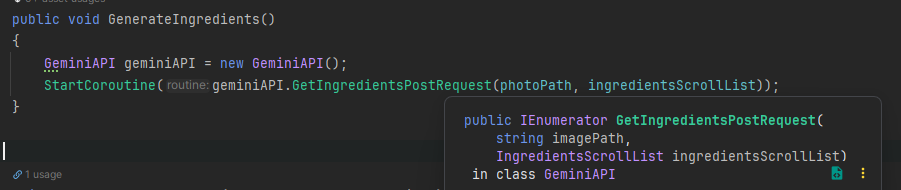
\includegraphics[width=0.8\textwidth,height=\textheight,keepaspectratio]{figures/chapter_1/UnityIEnumeratorCoroutine.png}
    \caption{Esempio di utilizzo di Coroutine}
\end{figure}

\subsection{Singleton}
Il \textbf{Singleton} è un design pattern che garantisce che una classe abbia una sola istanza e fornisce un punto di accesso globale a essa. Ci sono diversi modi per implementare un Singleton in C\#, tra cui l'implementazione normale e basica e quella thread-safe, utilizzata in questo progetto. La versione thread-safe garantisce che l'istanza sia creata in modo sicuro anche in un ambiente multi-thread, evitando problemi di concorrenza.\\Tralasciando la versione normale, la versione thread-safe utilizza un blocco chiamato nel codice \textbf{padlock} per garantire che solo un thread alla volta possa accedere alla creazione dell'istanza. 
\vspace{10cm}

\begin{lstlisting}[language=java]
public sealed class Singleton
{
    private static Singleton instance = null;
    private static readonly object padlock = new object();

    Singleton()
    {
    }

    public static Singleton Instance
    {
        get
        {
            lock (padlock)
            {
                if (instance == null)
                {
                    instance = new Singleton();
                }
                return instance;
            }
        }
    }
}


\end{lstlisting}
\cite{SingletonPatternCSharp}
\chapter{Utilizzo di Gemini come LLM e Spatial Understanding}
\pagestyle{plain}
In questo progetto è stato fatto uso di una LLM per il riconoscimento degli ingredienti e la successiva creazione di tre ricette. Fra tutte le LLM disponibili è stato scelto Gemini, la LLM sviluppata da Google, per la sua capacità di comprendere le immagini e l'API gratuita.

\section{Cosa è una LLM}
Un Large Language Model (LLM) è un modello di intelligenza artificiale in grado principalmente di riconoscere e generare testo. Gli LLM sono addestrati su grandi quantità di dati tramite l'uso del machine learning, nello specifico un particolare tipo di rete neurale chiamato Transformer. Per essere allenati in campi specifici, senza perdere il modello generato, viene utilizzato il fine-tuning, un processo che permette di specializzare il modello su un compito specifico.
Le informazioni che le LLM restituiscono sono affidabili quanto lo sono i dati che gli sono stati forniti durante l'allenamento, quindi se nei dati sono presenti delle informazioni sbagliate queste verranno date per giuste alle domande poste all'LLM. A volte invece gli LLM possono creare delle false informazioni dal nulla, questo fenomeno si chiama allucinazione, ad esempio nel 2022 venne chiesto a ChatGPT di creare un articolo sulla compagnia Tesla, l'LLM creò l'articolo, dove però la maggior parte delle informazioni erano inventate.\cite{LLMCloudflare}

Gli usi di una LLM sono vari, tra cui:
\begin{itemize}
    \item \textbf{Generazione di testo}: Creazione di email, blog, articoli e molto altro
    \item \textbf{Riassumere testo}: Riassumere lunghi articoli, notizie ma anche report aziendali
    \item \textbf{Generazione di codice}: Generare codice per la maggior parte di linguaggi di programmazione per aiutare il programmatore in compiti ripetitivi 
    \item \textbf{Traduzione}: Tradurre i testi in varie lingue, fornendo una traduzione accurata che prende nota anche del contesto delle parole
    \item \textbf{Accessibilità}: Aiutare le persone con disabilità a interagire con l'ambiente circostante, ad esempio generando descrizioni di immagini per persone non vedenti, tecnologia ancora in sviluppo con la recentissima versione di Gemini Live
\end{itemize}
\cite{LLMIBM} \cite{GeminiLiveBlog} \cite{GeminiLiveYoutube}

\section{Prompting}
I prompt sono utilizzati per interagire con le LLM, di solito sono delle domande, e in generale delle richieste testuali fatte dall'utente. Per ottenere le risposte volute nel prompt, oltre a porre la domanda o l'azione da fare, è necessario fornire, se necessario, il contesto, e se si vuole essere più specifici anche il formato della risposta, ad esempio un elenco puntato oppure un testo di poche righe. Da tenere a mente che però le LLM potrebbero non del tutto seguire le istruzioni fornite, soprattutto se si fanno richieste troppo specifiche come il numero di caratteri. \cite{PromptingNvidia} \cite{PromptingGoogle}

\section{Utilizzo di Gemini per Spatial Understanding}
Gemini offre la possibilità di utilizzare le immagini come input, e ottenere, oltre che una descrizione dell'immagine anche informazioni più specifiche e interessanti. Lo Spatial Understanding è una funzionalità che consente all'LLM di identificare gli oggetti presenti nell'immagine, restituendone i nomi e le relative coordinate spaziali. Si può provare questa funzionalità nel sito di Gemini Studio nella sezione "Build" sotto il nome di "Spatial Understanding". Nel nostro caso si darà alla LLM l'immagine di un tavolo o in generale di un piano in cui sono poggiati gli ingredienti e si chiederà all'LLM di restituire i nomi degli ingredienti e le relative posizioni.
\section{Utilizzo di Gemini come LLM}
Una volta ottenuti i nomi degli ingredienti, questi verranno dati a Gemini, a cui sarà chiesto di generare tre ricette utilizzando solo gli ingredienti forniti.


\chapter{Progettazione}
\pagestyle{plain}

\section{Casi D'uso}
\begin{figure}[H]
    \centering
    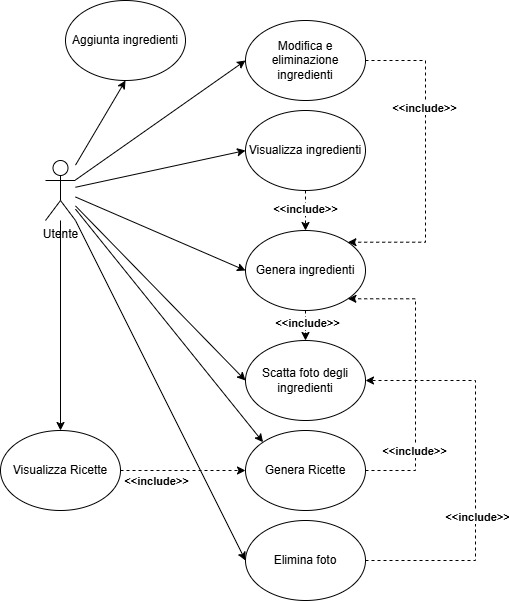
\includegraphics[width=0.8\textwidth,height=\textheight,keepaspectratio]{figures/chapter_1/use_case.jpg}
    \caption{}
    \label{fig:use_case}
\end{figure}

Lo use case in fig.\ref{fig:use_case} mostra lo scenario in cui l'utente ha già aperto entrambe le finestre dell'applicazione, quella per la fotocamera e generazione degli ingredienti e quella per la visualizzazione delle ricette. L'utente potrà scattare una foto ed eliminarla, generare gli ingredienti solo se la foto è stata scattata, aggiungere un ingrediente indipendentemente dalla foto, modificare un ingrediente già presente, generare tre ricette con gli ingredienti presenti e visualizzare le ricette generate.

\section{Architettura}
L'intera applicazione è standalone sul visore, quindi non necessita di un server per il funzionamento. Le uniche operazioni e calcoli che avvengono al di fuori del visore sono quelle che coinvolgono Google Gemini, che avvengono grazie a delle chiamate API in \textbf{POST}.
\section{Interfaccia grafica}
L'interfaccia è composta da due finestre, composte poi da più tabs, e un menu sempre visibile. Ogni finestra ha in alto una barra in cui è presente il nome della finesta e due bottoni posizionati a destra. Il bottone con il simbolo della "X" permette di chiudere la finestra, mentre quello con il simbolo della catena serve a bloccare la finestra nella posizione dove si trova o farsi seguire.
\subsection{Menu}
Il menu che vediamo nella figura \ref{fig:menu} è il menu principale che permette di mostrare e nascondere le finestre dell'applicazione, è composto da tre bottoni e una barra bianca sotto. Andando da sinistra verso destra troviamo il bottone per aprire la finestra per la fotocamera e generazione degli ingredienti, il bottone per vedere le ricette generate e il bottone per fare il pin della barra, in modo da tenerla ancorata nella posizione prefissata. Infatti di default la barra seguirà l'utente posizionandosi in basso in modo da non dar fastidio alle azioni con le altre finestre, sarà possibile spostarla utilizzando la barra bianca in basso.
\begin{figure}[H]
    \centering
    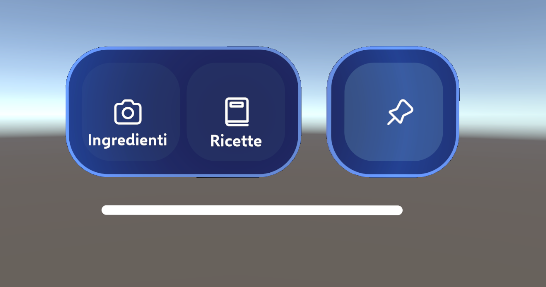
\includegraphics[width=\textwidth,height=\textheight,keepaspectratio]{figures/chapter_1/MENU_interfaccia.png}
    \caption{Menu principale dell'applicazione}
    \label{fig:menu}
\end{figure}
\subsection{Finestra per scatto della foto e generazione degli ingredienti}
Questa finestra è composta da due tabs, una per scattare la foto e visualizzarla come in fig.\ref{fig:camera}, l'altra per visualizzare gli ingredienti generati e apportare modifiche come in fig.\ref{fig:ingredienti}. Per cambiare da una tab all'altra sono presenti due bottoni in alto con in nome "Fotocamera" e "Ingredienti".
\subsubsection{Tab per la fotocamera}
Al centro troviamo la foto scattata, mentre a destra si trova un menu che ci permette di scattare la foto, eliminare la foto già scattata e generare gli ingredienti.
\begin{figure}[H]
    \centering
    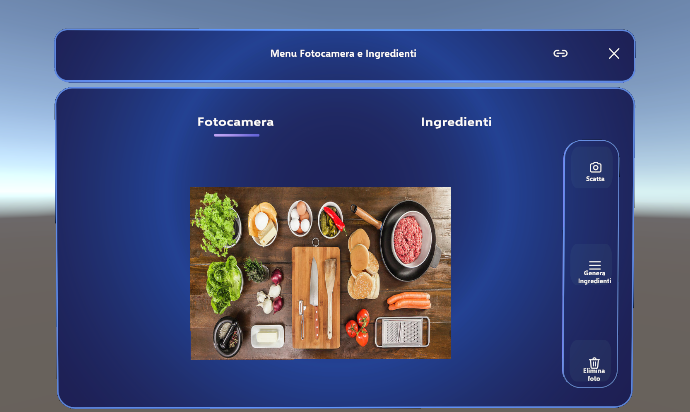
\includegraphics[width=\textwidth,height=\textheight,keepaspectratio]{figures/chapter_1/FOTOCAMERA_interfaccia.png}
    \caption{tab per la visualizzazione e scatto della foto}
    \label{fig:camera}
\end{figure}

\subsubsection{Tab per gli ingredienti}
Nella parte centrale si trova la scroll-list con gli ingredienti, a destra si trova il menu che permette di aggiungere un nuovo ingrediente o creare tre ricette con gli ingredienti presenti. Per la modifica di un ingrediente è necessario cliccare su di esso nella lista, in questo modo si aprirà una finestra di modifica come in fig.\ref{fig:modifica}.

\begin{figure}[H]
    \centering
    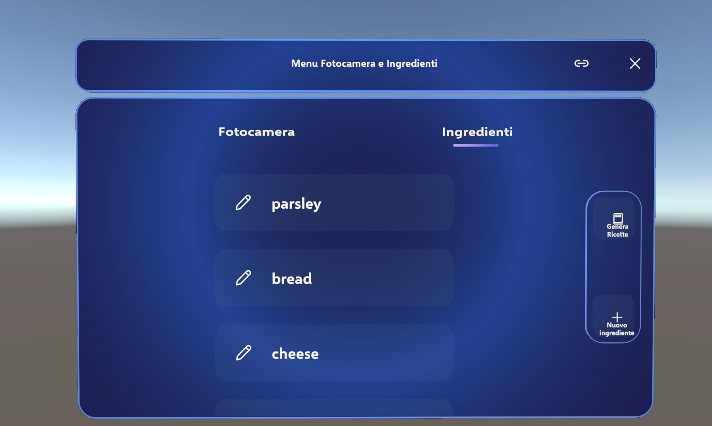
\includegraphics[width=\textwidth,height=\textheight,keepaspectratio]{figures/chapter_1/INGREDIENTI_interfaccia.png}
    \caption{Tab per la visualizzazione, inserimento  e modifica degli ingredienti}
    \label{fig:ingredienti}
\end{figure}

\begin{figure}[H]
    \centering
    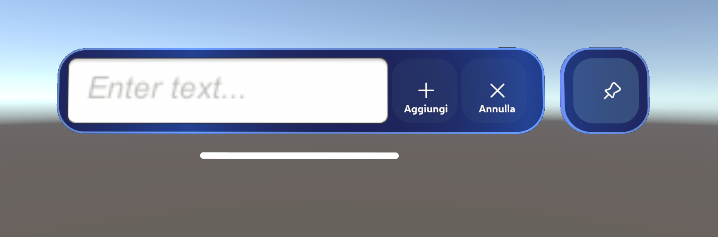
\includegraphics[width=\textwidth,height=\textheight,keepaspectratio]{figures/chapter_1/AGGIUNGI_interfaccia.png}
    \caption{Aggiunta di un ingrediente}
    \label{fig:aggiunta}
\end{figure}

\begin{figure}[H]
    \centering
    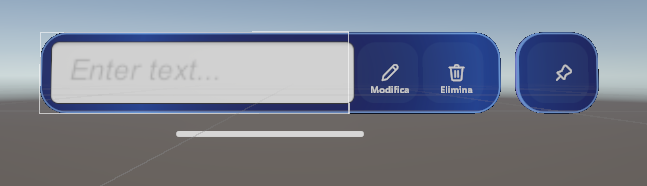
\includegraphics[width=\textwidth,height=\textheight,keepaspectratio]{figures/chapter_1/MODIFICA_interfaccia.png}
    \caption{Modifica di un ingrediente}
    \label{fig:modifica}
\end{figure}




\subsection{Finestra per visualizzazione delle ricette}
In alto troviamo un menu con tre bottoni che ci permettono di cambiare tab, ogni tab è composta da una scroll-list con le ricette generate. A destra troviamo un bottone che permette di generare nuove ricette.

\begin{figure}[H]
    \centering
    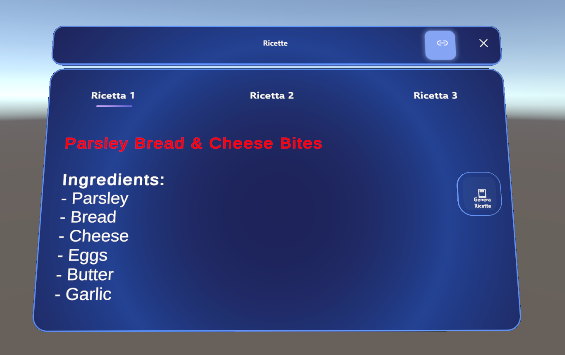
\includegraphics[width=\textwidth,height=\textheight,keepaspectratio]{figures/chapter_1/RICETTE_interfaccia.png}
    \caption{Interfaccia per la visualizzazione delle tre ricette}
    \label{fig:ricette}
\end{figure}



\section{Persistenza dei dati}
I dati vengono salvati in due file JSON, uno che contiene gli ingredienti e l'altro le ricette generate, la foto scattata invece viene salvata nella stessa direcory dei file JSON sotto un nome specifico. I nomi dei file si trovano all'interno di un file config, nella cartella StreamingAssets,  accessibile e leggibile come indicato in fig.\ref{fig:streamingAssets}

\begin{figure}[H]
    \centering
    
\includegraphics[width=\textwidth,height=\textheight,keepaspectratio]{figures/chapter_1/streamingAssets_CODICE.png}
    \caption{Codice per leggere il file di config}
    \label{fig:streamingAssets}
\end{figure}

Successivamente, grazie alla classe generica \textbf{FileHandler} possiamo serializzare e deserializzare i file JSON salvati, per modificarli o crearli. 
I file JSON  e l'immagine vengono salvati nel \textbf{persistentDataPath} come indicato in fig.\ref{fig:persistentDataPath}.

\begin{figure}[H]
    \centering
    
\includegraphics[width=\textwidth,height=\textheight,keepaspectratio]{figures/chapter_1/persistentDatapath_CODICE.png}
    \caption{Parte di codice che genera il path in cui salvare il file JSON}
    \label{fig:persistentDataPath}
\end{figure}
\chapter{Implementazione dell'applicazione}
\pagestyle{plain}


\section{Introduzione}
In questa sezione andremo a descrivere l'implementazione andando a dare uno sguardo più profondo al codice e successivamente anche alle problematiche riscontrate surante lo sviluppo con le relative soluzioni.


\section{Gemini API}
\subsection{Structured output}

\begin{wrapfigure}[8]{r}{0.30\textwidth} %this figure will be at the right
    \centering
    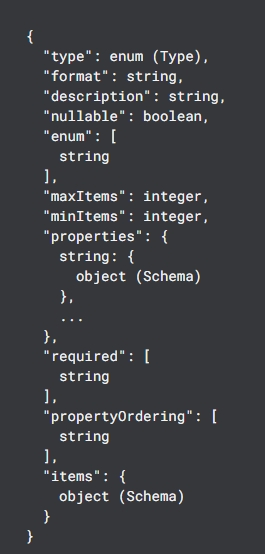
\includegraphics[width=0.30\textwidth]{figures/chapter_1/geminiPseudoSchema.png}
    \caption{Pseudo-JSON che rappresenta tutti i campi dello Schema}
\end{wrapfigure}

Lo Structured Output permette di farsi restituire da Gemini una risposta standardizzata, in questo caso un JSON, predefinita sotto forma di uno schema. Lo \textbf{Schema} supporta array, tipi e oggetti dentro i quali è possibile definire i tipi dei dati e i loro nomi. \cite{StructuredOutput}
I tipi nello \textbf{Schema} devono essere uno degli OpenAPI Data Types, oppure un'unione di questi tipi (utilizzando \texttt{anyOf}). Per ciascun tipo, è valido solo un determinato sottoinsieme di campi. Nella seguente lista viene riportata la corrispondenza tra ciascun tipo e il relativo insieme di campi validi:
\begin{itemize}
    \item \textbf{string}: \texttt{enum}, \texttt{format}, \texttt{nullable}
    \item \textbf{integer}: \texttt{format}, \texttt{minimum}, \texttt{maximum}, \texttt{enum}, \texttt{nullable}
    \item \textbf{number}: \texttt{format}, \texttt{minimum}, \texttt{maximum}, \texttt{enum}, \texttt{nullable}
    \item \textbf{boolean}: \texttt{nullable}
    \item \textbf{array}: \texttt{minItems}, \texttt{maxItems}, \texttt{items}, \texttt{nullable}
    \item \textbf{object}: \texttt{properties}, \texttt{required}, \texttt{propertyOrdering}, \texttt{nullable}
\end{itemize}

\begin{figure}[H]
    \centering
    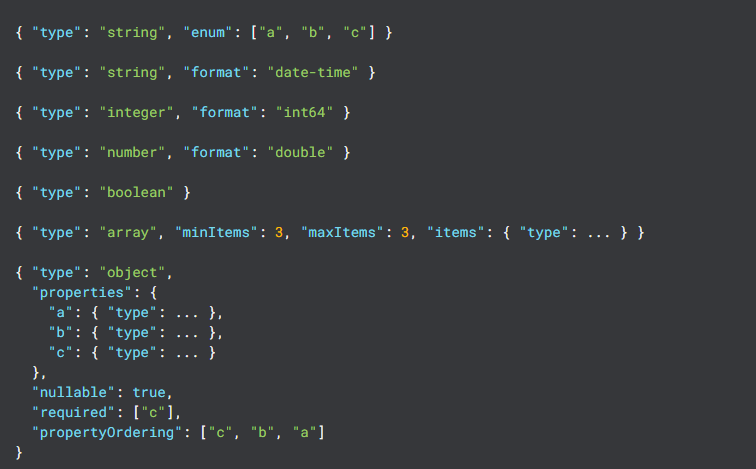
\includegraphics[width=0.8\textwidth,height=\textheight,keepaspectratio]{figures/chapter_1/GeminiSchema.png}
    \caption{Schemas di esempio}
\end{figure}

\subsection{Richieste POST}
Le richieste POST vengono fatte all'interno della classe \textbf{GeminiAPI}, che è anche la delegata al salvataggio dei dati ricevuti da Gemini in dei file JSON.

\begin{figure}[H]
    \centering
    
\includegraphics[width=0.8\textwidth,height=\textheight,keepaspectratio]{figures/chapter_1/GetIngredientsPostRequest.png}
    \caption{Funzione per generare gli ingredienti}
    \label{fig:getIngredientsPostRequest}
\end{figure}

\begin{figure}[H]
    \centering
    
\includegraphics[width=0.8\textwidth,height=\textheight,keepaspectratio]{figures/chapter_1/GetRecipesPostRequest.png}
    \caption{Funzione per generare le ricette}
    \label{fig:getRecipesPostRequest}
\end{figure}

\subsubsection{Generazione degli ingredienti}
Per generare gli ingredienti useremo la funzione della fig.\ref{fig:getIngredientsPostRequest}. Il payload della  POST richiede: 
\begin{itemize}
    \item Una immagine in formato \texttt{Base64}
    \item L'API Key e l'API url di Gemini
    \item Lo schema che definisce i campi che Gemini deve restituire
\end{itemize}

Per convertire l'imagine in formato \texttt{Base64} useremo la funzione \texttt{Convert.ToBase64String()} di C\#. 
\begin{figure}[H]
    \centering
    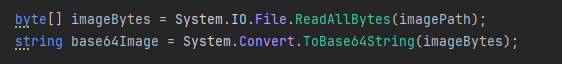
\includegraphics[width=0.8\textwidth,height=\textheight,keepaspectratio]{figures/chapter_1/base64.png}
    \caption{Lettura e conversione dell'immagine in Base64}
\end{figure}
\begin{figure}[H]
    \centering
    
\includegraphics[width=0.8\textwidth,height=\textheight,keepaspectratio]{figures/chapter_1/APIkey.png}
    \caption{Creazione dell'url per la richiesta POST}
    \label{fig:apiKey}
\end{figure}
L'API Key e l'url vengono letti dal file config come in fig.\ref{fig:apiKey}, che poi vengono messi all'interno del payload, insieme allo schema mostrato in fig.\ref{fig:structuredOutput} e all'immagine in formato \texttt{Base64} mostrato in fig.\ref{fig:imagePayload}.

\begin{figure}[H]
    \centering
    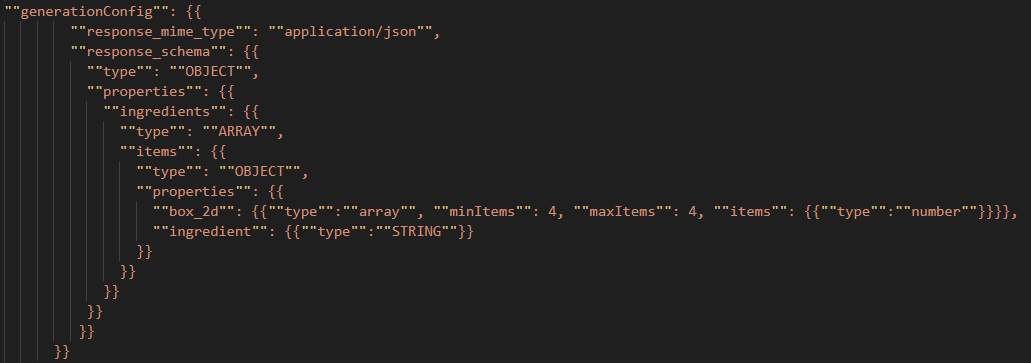
\includegraphics[width=0.8\textwidth,height=\textheight,keepaspectratio]{figures/chapter_1/StructuredOutput.png}
    \caption{Schema per la generazione degli ingredienti}
    \label{fig:structuredOutput}
\end{figure}
\begin{figure}[H]
    \centering
    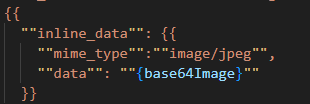
\includegraphics[width=0.5\textwidth,height=\textheight,keepaspectratio]{figures/chapter_1/imagePayload.png}
    \caption{Inserimento dell'immagine nel payload della richiesta POST}
    \label{fig:imagePayload}
\end{figure}
Infine viene effettuata la POST creando una nuova istanza della classe \textbf{UnityWebRequest}, convertendo il payload string in un array di byte per poi invocare il metodo \texttt{SendWebRequest()} per inviare la richiesta. Se la richiesta ha successo, Gemini risponderà con un JSON che contiene gli ingredienti, che verranno salvati in un file JSON.
\begin{figure}[H]
    \centering
    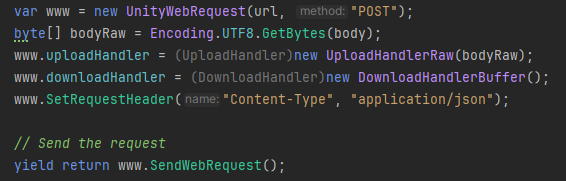
\includegraphics[width=0.6\textwidth,height=\textheight,keepaspectratio]{figures/chapter_1/richiestaPOST.png}
    \caption{Codice per effettuare la richiesta POST}
    \label{fig:postRequest}
\end{figure}

\subsubsection{Generazione delle ricette}
Per generare gli ingredienti useremo la funzione della fig.\ref{fig:getRecipesPostRequest}. In questo caso non ci servirà un'immagine ma la lista degli ingredienti, che verrà letta in un for e concatenata sotto un'unica stringa. La creazione dell'url e dell'API Key avviene come per la generazione degli ingredienti in fig.\ref{fig:apiKey}, ma lo Schema sarà diverso, come mostrato in fig.\ref{fig:recipeSchema}.

\begin{figure}[H]
    \centering
    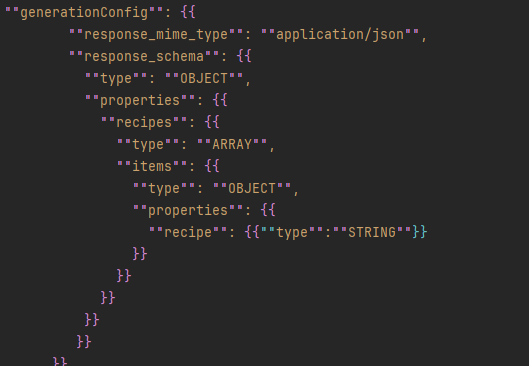
\includegraphics[width=0.6\textwidth,height=\textheight,keepaspectratio]{figures/chapter_1/recipeSchema.png}
    \caption{Schema per la generazione delle ricette}
    \label{fig:recipeSchema}
\end{figure}

Come possiamo facilmente notare lo schema è molto più semplice e richiede soltanto la restituzione di un array di oggetti, ognuno dei queli contiene una ricetta di tipo stringa.
Invece la richiesta testuale fatta è la seguente:
\begin{quote}
    \texttt{create three recipes only with the following ingredients: \{ingredientsConcat\}. Write it with tags compatible with TextMesh Pro, make the recipes titles colored in red, make the number of the instruction list colored in red, use bold in subtitles}
\end{quote}dove \texttt{ingredientsConcat} è la stringa che contiene tutti gli ingredienti separati da virgola.
L'invio della richiesta POST avviene come per la generazione degli ingredienti in fig.\ref{fig:postRequest}.

\section{File Handler}
la classe \textbf{FileHandler} è responsabile della lettura e scrittura e creazione dei file JSON. La particolarità è quella di essere una classe generica, in modo da poter serializzare tramite apposite classi serializzabili qualsiasi JSON.

\subsection{Classi Serializzabili}
Sono presenti quattro classi serializzabili, in particolare:
\begin{itemize}
    \item \textbf{ConfigJSON}: Serve a leggere il file di configurazione, dove sono salvati l'API Key, l'API URL di Gemini e i nomi dei file JSON da salvare e quello della foto.
    \item \textbf{GeminiResponseJSON}: Serve a leggere la risposta di Gemini che contiene gli ingredienti o le ricette e prendere i campi che ci interessano, in particolare il campo \texttt{text} tramite apposita funzione \texttt{GetText()}.
    \item \textbf{ListOfIngredientsJSON}: Utilizzata per salvare e leggere la lista degli ingredienti e ad assegnargli un ID univoco, che viene generato automaticamente quando si aggiunge un nuovo ingrediente.
    \item \textbf{ListOfRecipesJSON}: Utilizzata per salvare e leggere la lista delle ricette, che contiene un array di tipo \textbf{RecipesJSON}, ognuna delle quali contiene una stringa.
\end{itemize}

La separazione delle classi serializzabili da quelle del model permette di avere un codice più pulito e facilmente mantenibile, in quanto ogni classe ha una responsabilità ben definita.

\subsection{Metodi}
Sono presenti tre metodi:
\begin{itemize}
    \item \texttt{SaveJson(string jsonNameFile, T item)}: Salva un oggetto di tipo generico \textbf{T} nel file json con il nome passato tramite \textbf{jsonNameFile}. Il file viene creato se non esiste, altrimenti viene sovrascritto. Codice disponibile in fig.\ref{fig:saveJson}.
    \item \texttt{public T LoadJson(string jsonNameFile)}: deserializza un file JSON con il nome passato tramite \textbf{jsonNameFile} e restituisce un oggetto di tipo generico \textbf{T}. Se il file non esiste, ne viene creato uno vuoto e viene restituito un oggetto di tipo generico \textbf{T} vuoto. Codice disponibile in fig.\ref{fig:loadJson}.
    \item \texttt{CreateBlankFile(string filePath)}: Crea un file vuoto con il nome passato tramite \textbf{filePath}. Se il file esiste già, non viene creato nulla.
\end{itemize}

\begin{figure}[H]
    \centering
    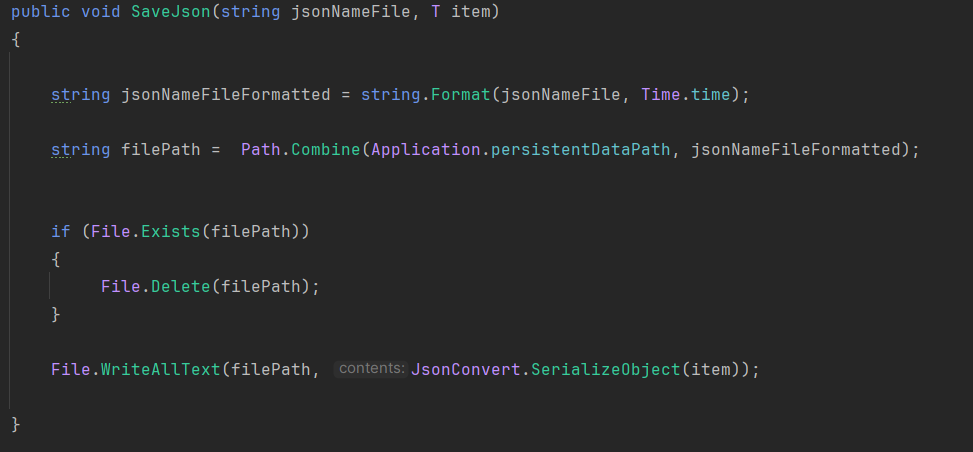
\includegraphics[width=0.6\textwidth,height=\textheight,keepaspectratio]{figures/chapter_1/saveJson_CODICE.png}
    \caption{Codice per effettuare il salvataggio del JSON}
    \label{fig:saveJson}
\end{figure}
\begin{figure}[H]
    \centering
    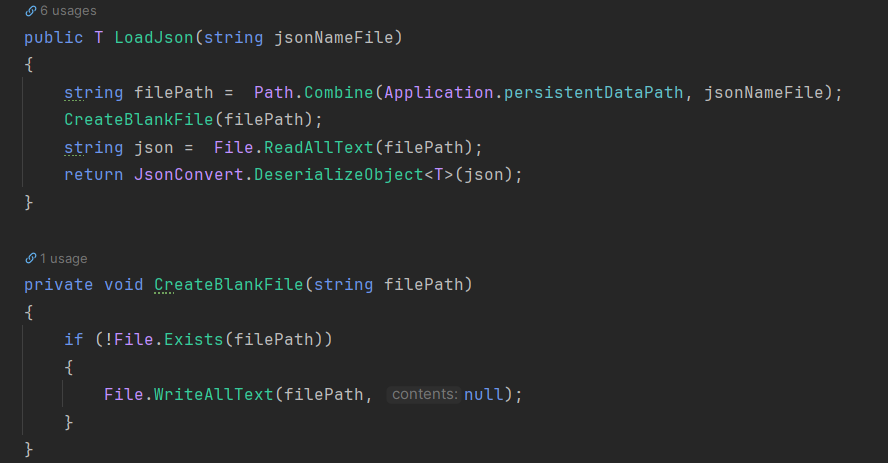
\includegraphics[width=0.6\textwidth,height=\textheight,keepaspectratio]{figures/chapter_1/LoadJson_CODICE.png}
    \caption{Codice per effettuare la deserializzazione del JSON}
    \label{fig:loadJson}
\end{figure}

\section{Scatto della foto}
Per scattare la foto usiamo la classe \textbf{PhotoShooter}, che utilizza la libreria \\ \textbf{UnityEngine.Windows.WebCam} di Unity per accedere alla fotocamera del dispositivo. La classe è responsabile della gestione della fotocamera, dello scatto della foto e del salvataggio dell'immagine in un file ed è implemantata tramite un singleton per garantire che ci sia una sola istanza della classe durante l'esecuzione dell'applicazione.
Sono presenti due funzioni principali:
\begin{itemize}
    \item \texttt{TakePhoto(string photoPath)}: controlla se la foto non esiste già, altrimenti la cancella e crea un processo asincrono per scattare e salvare la foto. Fig.\ref{fig:takePhoto}
    \item \texttt{DeletePhoto(string photoPath)}: cancella la foto scattata, se esiste. Fig.\ref{fig:deletePhoto}
\end{itemize}

\begin{figure}[H]
    \centering
    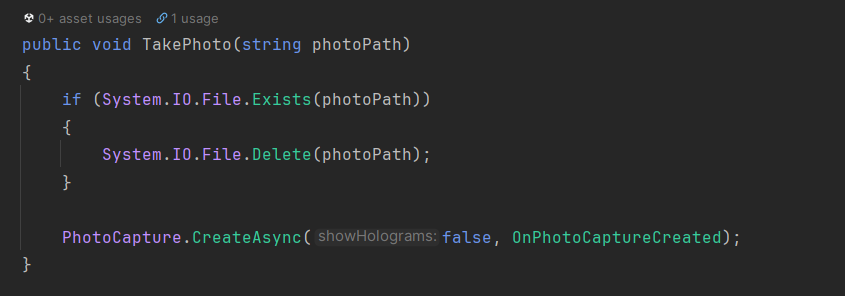
\includegraphics[width=0.6\textwidth,height=\textheight,keepaspectratio]{figures/chapter_1/TakePhoto_CODICE.png}
    \caption{Inizio funzione per lo scatto della foto}
    \label{fig:takePhoto}
\end{figure}
\begin{figure}[H]
    \centering
    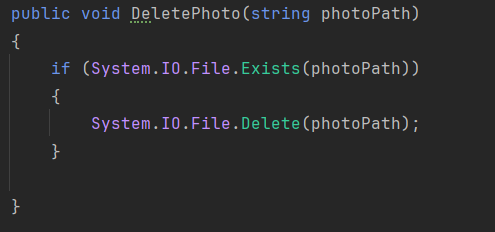
\includegraphics[width=0.6\textwidth,height=\textheight,keepaspectratio]{figures/chapter_1/DeletePhoto_CODICE.png}
    \caption{Codice per l'eliminazione della foto}
    \label{fig:deletePhoto}
\end{figure}
\begin{figure}[H]
    \centering
    \includegraphics[width=1\textwidth,height=\textheight,keepaspectratio]{figures/chapter_1/OnPhotoCaptureCreated_CODICE.png}
    \caption{Inizializzazione della fotocamera}
    \label{fig:onPhotoCaptureCreated}
\end{figure}
Nella figura \ref{fig:onPhotoCaptureCreated} il metodo \textbf{OnPhotoCaptureCreated} viene inizializzata la fotocamera con la massima risoluzione possibile e iniziata la cattura della foto in maniera asincrona utilizzando il metodo \textbf{OnPhotoModeStarted}

\begin{figure}[H]
    \centering
    \includegraphics[width=0.9\textwidth,height=\textheight,keepaspectratio]{figures/chapter_1/OnPhotoModeStarted_CODICE.png}
    \caption{Scatto della foto}
    \label{fig:onPhotoModeStarted}
\end{figure}
Nella figura \ref{fig:onPhotoModeStarted} il metodo \textbf{OnPhotoModeStarted} viene chiamato in maniera asincrona e tramite
\begin{lstlisting}[language=java]
    photoCaptureObject.TakePhotoAsync(filePath, PhotoCaptureFileOutputFormat.JPG, OnCapturedPhotoToDisk); 
\end{lstlisting}
    viene scattata la foto e utilizzato il metodo \textbf{OnCapturedPhotoToDisk} per salvare la foto su disco al path precedentemente definito dal \textbf{persistentDataPath}.

\begin{figure}[H]
    \centering
    \includegraphics[width=0.6\textwidth,height=\textheight,keepaspectratio]{figures/chapter_1/OnCapturedPhotoToDisk_CODICE.png}
    \caption{Salvataggio della foto su disco}
    \label{fig:onCapturedPhotoToDisk}
\end{figure}

In figura \ref{fig:onCapturedPhotoToDisk} il metodo \textbf{OnCapturedPhotoToDisk} è utilizzato per salvare la foto su disco, se l'operazione è compiuta con successo viene chiamato il metodo \textbf{OnStoppedPhotoMode} per terminare la modalità foto e rilasciare le risorse della fotocamera.


\begin{figure}[H]
    \centering
    \includegraphics[width=0.6\textwidth,height=\textheight,keepaspectratio]{figures/chapter_1/OnStoppedPhotoMode_CODICE.png}
    \caption{Procedura per terminare lo scatto della foto}
    \label{fig:onStoppedPhotoMode}
\end{figure}

In figura \ref{fig:onStoppedPhotoMode} il metodo \textbf{OnStoppedPhotoMode} viene chiamato per terminare la modalità foto e rilasciare le risorse della fotocamera, in particolare tramite \texttt{photoCaptureObject.Dispose()} il cui metodo \texttt{Dispose()} viene chiamato per arrestare l'istanza di \textbf{PhotoCapture}.

\section{Lista ingredienti}
Possiamo definire la lista degli ingredienti come uon dei più complessi elementi presenti nell'applicazione, in quanto è composta da dei prefab che vengono visualizzati in una lista, ognuno dei quali contiene il nome dell'ingrediente modificabile e eliminabile.
\subsection{Prefab}
Utilizzando il prefab \textbf{IngredientButtonRow} possiamo visualizzare gli ingredienti all'interno della lista, riusciendolo a generarlo quanti sono gli ingredianeti presenti nel file JSON.
\begin{figure}[H]
    \centering
    \includegraphics[width=1\textwidth,height=\textheight,keepaspectratio]{figures/chapter_1/prefab.png}
    \caption{Gerarchia del prefab IngredientButtonRow}
    \label{fig:prefab3D}
\end{figure}
Il prefab è un bottone al cui interno è presente un \textbf{TextMeshPro} per il nome dell'ingrediente, se cliccato verrà aperta la schermata di modifica del'ingrediente. 
Al prefab è assegnato uno script \textbf{IngredientButtonRow} che contiene i metodi per l'inizializzazione del prefab e il funzionamento generale.
\begin{figure}[H]
    \centering
    \includegraphics[width=0.9\textwidth,height=\textheight,keepaspectratio]{figures/chapter_1/prefab_CODICE.png}
    \caption{Classe IngredientButtonRow}
    \label{fig:prefabCodice}
\end{figure}

La variabile \textbf{TextFiels} è un riferimento al campo del prefab che contiene il nome dell'ingrediente, più in particolare è un campo serializzabile che viene visualizzato nell'Inspector di Unity, in modo da poterlo assegnare direttamente trascinando il componente, in questo caso il \textbf{TextMeshPro} del prefab, all'interno della variabile.
\subsection{Visualizzazione e spawn prefab}
\subsection{Aggiunta, modifica e cancellazione}

\section{Tastiera virtuale}
\section{Problematiche e soluzioni} 

\chapter{Conclusioni}
\pagestyle{plain}

\section{La mia esperienza con Unity e MRTK}
La mia esperienza con l'MRTK è stata in generale per lo più negativa, dettata da una scarsa documentazione ufficiale e anche poco materiale online di progetti di altri sviluppatori. I maggiori problemi si sono presentati quando ho dovuto costruire l'interfaccia grafica, in particolare nel far funzionare la scroll list e capire il funzionamento delle tab. Un'ulteriore difficoltà è stata reperire i prefab e gli esempi menzionati nella documentazione: spesso venivano mostrati come disponibili, ma risultavano difficilmente trovabili tramite fonti ufficiali. Anche il processo di compilazione per il visore non è dei migliori, con tempi di attesa per la prima build che si avvicinano alla mezz'ora, errori a fine compilazione abbastanza strani che si risolvono riavviando il pc, il visore o ricominciando da capo la compilazione, che come se non bastasse occupa uno spazio non indifferente sul disco e mi è capitato alcune volte di non aver spazio sufficente o addirittura di riempire completamente il disco. Altro punto a sfavore è la quantità di spazio richiesto per sviluppare l'applicazione, dato che bisogna installare componenti da Visual Studio Installer che pesano diversi GB. Altro problema che ho riscontrato, e che mi ha costetto a migrare l'intero progetto in un nuovo progetto Unity, è stato il fatto che installando dei componenti dalla Microsoft Mixed Reality Feature Tool, il progetto Unity non riusciva più a emulare dando errori di componenti mancanti, inoltre Unity, non permettendo di copiare e incollare la gerarchia senza creare dei prefab, ha reso più difficile e laborioso il processo di migrazione. Del resto la programmazione C\# in Unity è abbastanza lineare e ben documentata con un'ottima community online, che permette di risolvere la maggior parte dei problemi che si possono incontrare. Lato Hardware, gli Hololens sono un dispositivo molto interessante e con un potenziale enorme, anche se dotati di specifiche tecniche molto limitate nel 2025, punto a favore è che lo sviluppatore può controllarli in remoto accedendoci tramite IP, vedendo tutti i parametri vitali e anche una preview della telecamera, che permette di vedere cosa vede l'utente in tempo reale. Punto a sfavore invece è il FOV ("Field Of View") molto limitato e anche uno schermo che se non impostato correttamente potrebbe non avere i giusti colori o risultare sfocato.
\section{Sviluppi futuri dell'applicazione}
Si potrebbe migrare la parte di generazione di ingredienti e ricette su un server, così da poter creare un'applicazione multipiattaforma per qualsiasi dispositivo che supporti la realtà aumentata, dotando di un login l'utente in modo tale da poter andare a consultare le ricette salvate e gli ingredienti preferiti anche da altre piattaforme come smartphone o pc. Nel progetto attuale per gli Hololens si dovrebbe implementare la funzionalità di tracciare tramite le coordinate fornite da Gemini gli ingredienti nello spazio 3d, magari aggiungendo informazioni utili sui singoli ingredienti.

\section{Considerazioni finali}
L'esperienza di sviluppo con Unity e MRTK è stata complessa e ha richiesto un notevole impegno per superare le difficoltà legate alla documentazione e all'utilizzo dell'MRTK. Con lo sviluppo di questa applicazione ho capito il perchè non ci sono molti sviluppatori che si cimentano nello sviluppo di applicazioni per gli Hololens. Personalmente considero l'MRTK un progetto morto della Microsoft, che ha molti difetti e pochi pregi, surclassato da altri framework con una documentazione e processo di sviluppo migliore, come ad esempio quello di Meta utilizzato per lo sviluppo di applicazioni per il visori Meta Quest.

%   BACK MATTER
%   BIBLIOGRAPHY
\cleardoublepage
\addcontentsline{toc}{chapter}{Bibliografia}
\bibliography{include/3-back/bibliografia}

%   APPENDIX
%\cleardoublepage
%\appendix % to tell LaTeX that the following chapters are appendices
%\renewcommand\chaptername{Appendix}
\chapter{Appendix}

Lorem ipsum dolor sit amet, consectetur adipiscing elit. Vivamus at pulvinar nisi. Phasellus hendrerit, diam placerat interdum iaculis, mauris justo cursus risus, in viverra purus eros at ligula. Ut metus justo, consequat a tristique posuere, laoreet nec nibh. Etiam et scelerisque mauris. Phasellus vel massa magna. Ut non neque id tortor pharetra bibendum vitae sit amet nisi. Duis nec quam quam, sed euismod justo. Pellentesque eu tellus vitae ante tempus malesuada. Nunc accumsan, quam in congue consequat, lectus lectus dapibus erat, id aliquet urna neque at massa. Nulla facilisi. Morbi ullamcorper eleifend posuere. Donec libero leo, faucibus nec bibendum at, mattis et urna. Proin consectetur, nunc ut imperdiet lobortis, magna neque tincidunt lectus, id iaculis nisi justo id nibh. Pellentesque vel sem in erat vulputate faucibus molestie ut lorem.

Quisque tristique urna in lorem laoreet at laoreet quam congue. Donec dolor turpis, blandit non imperdiet aliquet, blandit et felis. In lorem nisi, pretium sit amet vestibulum sed, tempus et sem. Proin non ante turpis. Nulla imperdiet fringilla convallis. Vivamus vel bibendum nisl. Pellentesque justo lectus, molestie vel luctus sed, lobortis in libero. Nulla facilisi. Aliquam erat volutpat. Suspendisse vitae nunc nunc. Sed aliquet est suscipit sapien rhoncus non adipiscing nibh consequat. Aliquam metus urna, faucibus eu vulputate non, luctus eu justo.

Donec urna leo, vulputate vitae porta eu, vehicula blandit libero. Phasellus eget massa et leo condimentum mollis. Nullam molestie, justo at pellentesque vulputate, sapien velit ornare diam, nec gravida lacus augue non diam. Integer mattis lacus id libero ultrices sit amet mollis neque molestie. Integer ut leo eget mi volutpat congue. Vivamus sodales, turpis id venenatis placerat, tellus purus adipiscing magna, eu aliquam nibh dolor id nibh. Pellentesque habitant morbi tristique senectus et netus et malesuada fames ac turpis egestas. Sed cursus convallis quam nec vehicula. Sed vulputate neque eget odio fringilla ac sodales urna feugiat.

Phasellus nisi quam, volutpat non ullamcorper eget, congue fringilla leo. Cras et erat et nibh placerat commodo id ornare est. Nulla facilisi. Aenean pulvinar scelerisque eros eget interdum. Nunc pulvinar magna ut felis varius in hendrerit dolor accumsan. Nunc pellentesque magna quis magna bibendum non laoreet erat tincidunt. Nulla facilisi.

Duis eget massa sem, gravida interdum ipsum. Nulla nunc nisl, hendrerit sit amet commodo vel, varius id tellus. Lorem ipsum dolor sit amet, consectetur adipiscing elit. Nunc ac dolor est. Suspendisse ultrices tincidunt metus eget accumsan. Nullam facilisis, justo vitae convallis sollicitudin, eros augue malesuada metus, nec sagittis diam nibh ut sapien. Duis blandit lectus vitae lorem aliquam nec euismod nisi volutpat. Vestibulum ornare dictum tortor, at faucibus justo tempor non. Nulla facilisi. Cras non massa nunc, eget euismod purus. Nunc metus ipsum, euismod a consectetur vel, hendrerit nec nunc.


Quisque tristique urna in lorem laoreet at laoreet quam congue. Donec dolor turpis, blandit non imperdiet aliquet, blandit et felis. In lorem nisi, pretium sit amet vestibulum sed, tempus et sem. Proin non ante turpis. Nulla imperdiet fringilla convallis. Vivamus vel bibendum nisl. Pellentesque justo lectus, molestie vel luctus sed, lobortis in libero. Nulla facilisi. Aliquam erat volutpat. Suspendisse vitae nunc nunc. Sed aliquet est suscipit sapien rhoncus non adipiscing nibh consequat. Aliquam metus urna, faucibus eu vulputate non, luctus eu justo.

Donec urna leo, vulputate vitae porta eu, vehicula blandit libero. Phasellus eget massa et leo condimentum mollis. Nullam molestie, justo at pellentesque vulputate, sapien velit ornare diam, nec gravida lacus augue non diam. Integer mattis lacus id libero ultrices sit amet mollis neque molestie. Integer ut leo eget mi volutpat congue. Vivamus sodales, turpis id venenatis placerat, tellus purus adipiscing magna, eu aliquam nibh dolor id nibh. Pellentesque habitant morbi tristique senectus et netus et malesuada fames ac turpis egestas. Sed cursus convallis quam nec vehicula. Sed vulputate neque eget odio fringilla ac sodales urna feugiat.


%   ACKNOWLEDGEMENTS
%\cleardoublepage
%\pagenumbering{gobble}
%\thispagestyle{plain}			% Supress header
\section*{Acknowledgements}
Lorem ipsum dolor sit amet, consectetur adipisicing elit, sed do eiusmod tempor incididunt ut labore et dolore magna aliqua. Ut enim ad minim veniam, quis nostrud exercitation ullamco laboris nisi ut aliquip ex ea commodo consequat. Duis aute irure dolor in reprehenderit in voluptate velit esse cillum dolore eu fugiat nulla pariatur. Excepteur sint occaecat cupidatat non proident, sunt in culpa qui officia deserunt mollit anim id est laborum.

\vspace{1.5cm}
\hfill
Name Familyname, Rome, Month Year

\newpage				% Create empty back of side
\thispagestyle{empty}
\mbox{}

\end{document} 